\cotefile{11}
\scanpage{43}
\margin{42}
\mspage{-3.7-}

(identifying $\mathbb{A}_R$ as $\mathbb{A}^{n\nu-n}$), so that $(\mathbb{A}^{n\nu-n},\phi_R)$ is a geometric quotient of $U_R$ by $\mathrm{PGL}(n)$. Moreover, recall that
\[
\sigma_R:\mathbb{A}^{n\nu-n}\longrightarrow U_R
\]
is a global section for $\phi_R$. The following is obvious:

\uline{Corollary 3.2}: Suppose $U\subset U_R$ is any invariant open subset. Then $U\cong\mathrm{PGL}(n)\times\sigma_R^{-1}(U)$, the isomorphism being compatible with the obvious operations of $\mathrm{PGL}(n)$.

To illustrate these results, which may be somewhat obscured by the cumbersome machinery of $R$-partitions, look at the case $\nu=1$, $S_1=\{0,1,\ldots,n\}$. The proposition is then the classical result that $n+2$ points in ``general'' position in $\mathbb{P}_n$ can be normalized to the canonical points $(1,0,\ldots,0)$, $(0,1,\ldots,0),\ldots,(0,0,\ldots,1)$, and $(1,1,\ldots,1)$ by a unique projective transformation. To give a second example, suppose $n=2$, $\nu=2$,
\[
S_1=\{0,1\},\quad S_2=\{1,2\}.
\]
The proposition asserts that, given 5 points $P_0,P_1,P_2$, $P_3$ and $P_4$ in the plane, suppose $P_0,P_1$ and $P_2$ are not collinear, that $P_3$ is not on the line $\overline{P_0P_2}$ or the line $\overline{P_1P_2}$ and that $P_4$ is not on the line $\overline{P_0P_1}$ or $\overline{P_0P_2}$: then we can uniquely normalize $P_0,P_1,P_2$ to $(1,0,0)$, $(0,1,0)$ and $(0,0,1)$ respectively, and normalize $P_3$ to $(1,1,a)$, $P_4$ to $(b,1,1)$ by a suitable projective transformation. (cf. Figure 3, where $Q_3=(1,1,0)$, $Q_4=(0,1,1)$).

\scanpage{44}

Variantes évidentes avec des variétés topologiques compactes.
On peut prendre pour $k$ un anneau \inserted{(\unsure{pas corps})}, lorsqu'on a une théorie de \unsure{cohomologie|coh. alg.} à coefficients dans $k$ \deleted{\unsure{qui satisfait}} \inserted{telle que} \deleted{\unsure{Poincaré}} $H^*(X)$ satisfait à Poincaré \deleted{\illegible{1}} (pas seulement mod torsion\ldots).

2) Considérons un autre foncteur de $\unsure{\mathcal{V}}$ en les anneaux bivariants \unsure{jaugés}, tel le foncteur $A^*(X)$ (anneau de Chow, \deleted{\unsure{gradué}} \unsure{jaugé} par le \uline{degré} des cycles de degré max), ou un foncteur quotient (tels les groupes de cycles mod équiv. numérique, homologique, $\unsure{\checkmark^{\tau}}$ algébrique, Picard, Albanese\ldots). On trouve un anneau bivariant \unsure{jaugé} simplicial, qui n'a plus aucune tendance à être spécial, et dont les composantes n'ont pas \unsure{trop} envie d'être de Poincaré\ldots

On peut tensoriser par $\mathbb{Q}$\ldots

3) On peut prendre $K(X)$ [\unsure{jaugé} par $\chi$], considéré comme gradué de degré 0\ldots

\figure{\begin{tikzpicture}\draw (0,0)--(5.7,0);\end{tikzpicture}}
Formalisme des correspondances. Soit $C\in A(I\amalg I')$. On va lui associer une application
\[
x\unsure{\mapstochar\relbar|\mapsto} C(x)=C.x:\quad A(I)\longrightarrow A(I')
\]
Ce sera le composé (où $\alpha:I-I\amalg I'$, $\alpha':I'-I\amalg I'$)
\diagram{
\begin{tikzcd}
A(I) \arrow[r,"\unsure{\alpha^*}"] & A(I\amalg I') \arrow[r,"y\mapsto Cy"] & A(I\amalg I') \arrow[r,"\alpha'_*"] & A(I')
\end{tikzcd}
}
\margin{il y a un choix: prendre $Cy$ ou $yC$ !}

Ces actions sont connues quand on connaît, en plus des lois d'\uline{anneaux} des $A(\unsure{\cdot})$, les $\alpha^*$ et $\alpha_*$ pour $\alpha:I\unsure{\lhook\joinrel-|\hookrightarrow}J$ une injection [il suffit avec $\operatorname{card}(J)=\operatorname{card}(I)+1$, i.e $\alpha$ un ``opérateur face''].
\margin{43}

\scanpage{45}
\margin{44}
\mspage{-3.6-}

for every $j\in\{0,1,\ldots,n\}$.

Note that $\lambda_j$ is a section of $L_j\otimes L_{\mu(1)}^{-1}$ over the open set $U_R$. We now define
\[
\phi:U_R\longrightarrow\mathrm{PGL}(n)\times\mathbb{A}_R
\]
by its two components $p_1\circ\phi$ and $p_2\circ\phi$. The projective group $\mathrm{PGL}(n)$, is, by definition, the affine open subset of
\[
\mathbb{P}_{n^2+2n}=\operatorname{Proj}\mathbb{Z}[a_{00},\ldots,a_{0n};\ a_{10},\ldots,a_{1n};\ \ldots;\ a_{n0},\ldots,a_{nn}]
\]
where $\det(a_{ij})\ne0$. Therefore $p_1\circ\phi$ is determined by
\[
\begin{aligned}
(p_1\circ\phi)^*(\underline{o}_{\mathbb{P}}(1))&=L_{\mu(1)}\\
(p_1\circ\phi)^*(a_{ij})&=x_i^{(j)}\otimes(-1)^j\lambda_j^{-1}.
\end{aligned}
\]

Finally the morphism $p_2\circ\phi$ into affine space is determined by:
\[
(p_2\circ\unsure{\psi|\phi})^*(x_i^{(n+k)})
=\frac{D_{0,1,\ldots,\widehat{i},\ldots,n,n+k}}{D_{0,1,\ldots,\widehat{\mu(k)},\ldots,n,n+k}}
\cdot\frac{\lambda_i}{\lambda_{\mu(k)}}
\]
(It should be noted that the expression on the right is actually a section of $\underline{o}_{\mathbb{A}_R}$). Modulo the mechanical verifications that remain, this proves the Proposition. \uline{QED}

Of the morphisms constructed in the course of the above proof, it is useful to \deleted{\unsure{let}} fix the notation:
\[
\phi_R=p_2\circ\phi:U_R\longrightarrow\mathbb{A}^{n\nu-n}
\]

\scanpage{46}

Posons $A(I';I)$ au lieu de $A(I\amalg I')$.
\margin{\deleted{\unsure{Hom}} (\unsure{Alg des corr.} de $I:I'$)}
On va définir une application naturelle $k$-bilinéaire
\[
A(I'',I')\times A(I',I)\overset{\unsure{\gamma}}{\longmapsto}A(I'',I)
\]
notée $(v,u)\longmapsto v\circ u$, et définie par
\[
v\circ u=p_{31*}\bigl(p_{21}^*(u)\,p_{32}^*(v)\bigr)
\]
\margin{
\diagram{
\begin{tikzcd}
& X^{I\amalg I'} \arrow[dl,"\alpha"'] \arrow[dr,"\alpha'"] &\\
X^I && X^{I'}
\end{tikzcd}
}
}

Ceci posé, si $\widetilde{u}:A(I)-A(I')$, \deleted{$\unsure{v}$}\ldots\ on vérifie la formule
\[
\widetilde{v\circ u}=\widetilde v\circ\widetilde u
\]
\margin{
\diagram{
\begin{tikzcd}[column sep=small,row sep=small]
&& X^{I\amalg I'\amalg I''} \arrow[dll,"p_{21}"'] \arrow[dd,"p_{31}"] \arrow[drr,"p_{32}"] &&\\
X^{I\amalg I'} \arrow[dd,"\gamma"'] \arrow[ddr,"\gamma'"] &&&& X^{I'\amalg I''} \arrow[ddl,"\alpha'"'] \arrow[dd,"\alpha''"]\\
&& X^{I\amalg I''} \arrow[ddl,no head,"\beta"'] \arrow[ddr,no head,"\beta''"] &&\\
X^I & X^{I'} && X^{I'} & X^{I''}\\
& X^I && X^{I''} &
\end{tikzcd}
}
}

En effet, on a
\[
\begin{aligned}
\widetilde{(v\circ u)}(x)
&\overset{\text{déf de }\widetilde{\deleted{\unsure{u}}}}{=}
\deleted{\unsure{p_{3*}}}\,
\beta''_*\bigl[(v\circ u)\,\beta^*(x)\bigr]\\
&\overset{\text{déf de }v\circ u}{=}
\beta''_*\Bigl[\underbrace{p_{31*}\bigl(p_{21}^*(u)\,p_{32}^*(v)\bigr)\,\beta^*(x)}
_{\Vert\ -\ \text{form. de proj}}\Bigr]\\
&=p_{31*}\bigl(p_{21}^*(u)\,p_{32}^*(v)\,
\underbrace{p_{31}^*\beta^*(x)}_{p_1^*(x)}\bigr)\\
&\overset{\text{transit}}{=}p_{3*}\bigl(p_{21}^*(u)\,p_{32}^*(v)\,p_1^*(x)\bigr)\\
&\deleted{\overset{\text{projection}}{=}p_{3*}\bigl(p_{21}^*(u)\,p_{32}^*(\unsure{v})\bigr)x}
\end{aligned}
\]

\[
\begin{aligned}
\widetilde v(\widetilde u(x))
&\overset{\text{déf }\widetilde v}{=}
\deleted{\unsure{\alpha''_*(\widetilde u(x))}}\,
\alpha''_*\bigl(v\,\alpha'^*(\widetilde u(x))\bigr)\\
&\overset{\text{déf }\widetilde u}{=}
\alpha''_*\bigl(v\,\underbrace{\alpha'^*\bigl(\gamma'_*(u\,\gamma^*(x))\bigr)}
_{\Vert\ \text{ici on a}}\bigr)\ \deleted{\unsure{=}}\\
&\hspace{2em}\deleted{\unsure{\alpha'_*(x)}}\\
&\hspace{2em}p_{32*}\bigl(p_{21}^*(u\,\gamma^*(x))\bigr)
=p_{32*}\bigl(p_{21}^*(u)\,\underbrace{p_{21}^*\gamma^*(x)}_{p_1^*(x)}\bigr)
\end{aligned}
\]
\margin{\figure{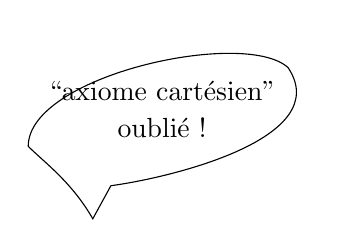
\begin{tikzpicture}
\node at (1.7,.85) {``axiome cartésien''};
\node at (1.7,.38) {oublié !};
\draw (0,.15) .. controls (0,1.05) and (2.75,1.65) .. (3.3,1.15)
.. controls (3.9,.25) and (1.8,-.25) .. (1.05,-.35)
--(.82,-.77) .. controls (.55,-.3) and (.2,-.05) .. (0,.15);
\end{tikzpicture}}}
\margin{
\diagram{
\begin{tikzcd}[column sep=small]
& X^{I\amalg I'\amalg I''} \arrow[dl,"p_{21}"'] \arrow[dr,"p_{32}"] &\\
X^{I\amalg I'} \arrow[dr,"\gamma'"'] && X^{I'\amalg I''} \arrow[dl,"\alpha'"] \arrow[dr,no head,"\alpha''"] &\\
& X^{I'} && X^{I''}
\end{tikzcd}
}
}
\[
\begin{aligned}
&=\alpha''_*\bigl(\underbrace{v\,p_{32*}\bigl(p_{21}^*(u)\,p_1^*(x)\bigr)}
_{\Vert\ \text{formule de projection, }\uline{\text{mod signe}}}\bigr)=\\
&\deleted{=\unsure{\alpha}}\quad
\underbrace{\alpha''_*p_{32*}}_{\Vert}\bigl(p_{32}^*(v)\,p_{21}^*(u)\,p_1^*(x)\bigr)\\
&\hspace{4em}p_{3*}\bigl(p_{32}^*(v)\,p_{21}^*(u)\,p_1^*(x)\bigr)
\end{aligned}
\]
\margin{OK mod \uline{signes}, à \unsure{faire} \uline{attention}}
\margin{45}

\scanpage{47}
\margin{46}
\mspage{-3.4-}

space. Then there is a $\mathrm{PGL}(n)$-linear isomorphism:
\[
(*)\qquad U_R\cong\mathrm{PGL}(n)\times\mathbb{A}^{n\nu-n}
\]
Hence $U_R$ is a globally trivial principal fibre bundle with respect to the action of $\mathrm{PGL}(n)$, with base space $\mathbb{A}^{n\nu-n}$.

\uline{Proof}: We shall construct morphisms from the left hand side of $(*)$ to the right, and vice versa, leaving it to the reader to check that they are mutually inverse. The morphisms will be obviously $\mathrm{PGL}(n)$-linear. First of all, we identify $\mathbb{A}^{n\nu-n}$ with the scheme:
\[
\mathbb{A}_R=\operatorname{Spec}
\frac{\mathbb{Z}[x_0^{(n+1)},\ldots,x_n^{(n+1)};\ x_0^{(n+2)},\ldots,x_n^{(n+2)};\ldots;\ x_0^{(n+\nu)},\ldots,x_n^{(n+\nu)}]}
{\text{Ideal generated by }\{x_i^{(n+k)}-1\mid i\in S_k\}}
\]
since both are affine spaces of dimension $n\nu-n$. Then a morphism
\[
\unsure{S_R|s_R}:\mathbb{A}_R\longrightarrow U_R
\]
is defined by the collection of composite morphisms
\diagram{
\begin{tikzcd}[column sep=small]
\unsure{S_i|s_i}: \mathbb{A}_R \arrow[r,"\unsure{S|s}"] & U_R\subset(\mathbb{P}_n)^{n+\nu+1} \arrow[r,"p_i"] & \mathbb{P}_n
\end{tikzcd}
}
and $\unsure{S_i|s_i}$ is defined by the conditions (cf. EGA 2, 4.2.3):
\[
\begin{aligned}
\unsure{S_i|s_i}^*(\underline{o}(1))&\cong\underline{o}_{\mathbb{A}}\\
\unsure{S_i|s_i}^*(X_j)&=\delta_{ij}\quad\text{if }0\leq i\leq n\\
\unsure{S_i|s_i}^*(X_j)&=x_j^{(i)}\quad\text{if }n+1\leq i\leq m
\end{aligned}
\]

\scanpage{48}

On va définir aussi
\[
\Delta_I\in A(I\amalg I)
\]
qui sera tel que
\[
\widetilde{\unsure{\delta|\Delta}}_I(x)=x\qquad(x\in A(I))
\qquad\text{i.e.}\quad\widetilde{\unsure{\delta|\Delta}}_I=\operatorname{id}_{A(I)}.
\]
Pour le voir, on \deleted{définit} considère $\delta:I\amalg I-I$, d'où
\[
\delta^{\deleted{\unsure{*}}}_*:A(I)-A(I\amalg I),
\]
on pose
\[
\Delta_I=\delta_*(1)
\]
On aura (\unsure{écrivant} $\Delta$ au lieu de $\Delta_I$
\margin{
\diagram{
\begin{tikzcd}
& X^I \arrow[d,no head,"\delta"] &\\
& X^{I\amalg I} \arrow[dl,"p_1"'] \arrow[dr,"p_2"] &\\
X^I && X^I
\end{tikzcd}
}
}
\[
\begin{aligned}
\widetilde\Delta(x)&\overset{\text{déf}}{=}p_{2*}\bigl(\Delta\,p_1^*(x)\bigr)\\
&=p_{2*}\bigl(\underbrace{\delta_*(1)\,p_1^*(x)}
_{\substack{\Vert\\ \unsure{\text{pr.}}\ \delta_*(\delta^*p_1^*(x))=\delta_*(x)}}\bigr)\\
&=p_{2*}\delta_*(x)=x
\end{aligned}
\]

Il faut encore \unsure{définir|vérifier} l'associativité de l'opération $\bullet$, et le fait que les $\unsure{\delta|\Delta}_I$ jouent le rôle d'unités. On voit que sous ces conditions,
\margin{47}

\scanpage{49}
\margin{48}
\mspage{-3.3-}

$0\leq\alpha_i\leq m$, let
\[
D_{\alpha_0,\ldots,\alpha_n}=\det_{0\leq i,j\leq n}\bigl[X_i^{(\alpha_j)}\bigr]
\]
be the section of $L_{\alpha_0}\otimes\cdots\otimes L_{\alpha_n}$ obtained by addition and tensor product as in the determinant. It is evident that $D_{\alpha_0,\ldots,\alpha_n}$ is an \uline{invariant} section of $L_{\alpha_0}\otimes\cdots\otimes L_{\alpha_n}$. The non-vanishing of suitable $D$'s defines the open sets we are looking for.

\uline{Definition 3.2}: An \uline{$R$-partition} of $\{0,1,\ldots,n\}$ is an ordered set of subsets $S_1,S_2,\ldots,S_\nu$ of $\{0,1,\ldots,n\}$ such that

(i) $S_i\cap(S_{i-1}\cup\cdots\cup S_2\cup S_1)$ consists of exactly one integer, for $2\leq i\leq\nu$,

(ii) $\displaystyle\bigcup_{i=1}^{\nu}S_i=\{0,1,\ldots,n\}$,

\uline{Definition 3.3}: Given an $R$-partition $R=\{S_1,\ldots,S_\nu\}$, let $U_R\subset(\mathbb{P}_n)^{n+\nu+1}$ be the open subset defined by
\[
\text{(i)}\quad D_{0,1,\ldots,n}\ne0,
\]
(ii) for all $k$ between 1 and $\nu$, and for all $i\in S_k$
\[
D_{0,1,\ldots,\widehat i,\ldots,n,n+k}\ne0
\]

Not only is $U_R$ affine, but the whole structure of the action of $\mathrm{PGL}(n)$ on $U_R$ can be described explicitly:

\uline{Proposition 3.1}: Let $R=\{S_1,\ldots,S_\nu\}$ be an $R$-partition of $\{0,1,\ldots,n\}$. Let $\mathrm{PGL}(n)$ act on $\mathrm{PGL}(n)\times\mathbb{A}^{n\nu-n}$ by the product of left translation on itself and the trivial action on the affine

\scanpage{51}

Sous-algèbres tautologiques de $H^*(X^n)$.

\textcircled{1}\quad\uline{$H^*(X)$}
\deleted{\unsure{degré}}

\uline{générateurs}\quad $\unsure{y|\eta}\in H^{\unsure{n|m}}(X)$

\uline{relations}\quad $\unsure{y|\eta}^2=0$

\uline{base}
\diagram{$
\begin{array}{ll}
\text{deg. }0&1\\
\text{deg. }\unsure{n|m}&\unsure{y|\eta}
\end{array}
$}

\textcircled{2}\quad\uline{$H^*(X\times X)$}

\uline{générateurs}:
\[
\unsure{y|\eta}\otimes1=\unsure{y|\eta}_1\ \deleted{\unsure{*}},\quad
1\otimes\unsure{y|\eta}=\unsure{y|\eta}_2,\quad
\delta\in H^{\unsure{n|m}}(X)
\]

\uline{relations}
\[
\unsure{y|\eta}_1^2=\unsure{y|\eta}_2^2=0,\quad
\unsure{y|\eta}_1\unsure{y|\eta}_2=\unsure{y|\eta}_1\delta=\unsure{y|\eta}_2\delta;\quad
\delta^2=\chi\,\unsure{y|\eta}_1\unsure{y|\eta}_2
\]
\margin{($\chi\in\mathbb Z$ la car. d'EP)}

\uline{base}
\diagram{$
\begin{array}{ll}
\text{deg }0&1\\
\text{deg }\unsure{n|m}&\unsure{y|\eta}_1,\unsure{y|\eta}_2,\delta\\
\text{deg }2\unsure{n|m}&\unsure{y|\eta}_1\unsure{y|\eta}_2\unsure{y|\eta}_3
\end{array}
$}

\textcircled{3}\quad $H^*(X\times X\times X)$

\uline{générateurs}
\[
\begin{array}{ll}
\text{deg. }\unsure{n|m}:&
\unsure{y|\eta}\otimes1\otimes1=\unsure{y|\eta}_1,\quad
1\otimes\unsure{y|\eta}\otimes1=\unsure{y|\eta}_2,\quad
1\otimes1\otimes\unsure{y|\eta}=\unsure{y|\eta}_3,\quad
\delta_{12}=\delta\otimes1,\delta_{23},\delta_{31}\\
\text{deg }2\unsure{n|m}&\delta
\end{array}
\]

\uline{relations}
\[
\left\{
\begin{aligned}
&\unsure{y|\eta}_1^2=\unsure{y|\eta}_2^2=\unsure{y|\eta}_3^2=0\\
&\delta_{12}^2=\chi\unsure{y|\eta}_1\unsure{y|\eta}_2,\quad
\delta_{23}^2=\chi\unsure{y|\eta}_2\unsure{y|\eta}_3,\quad
\delta_{31}^2=\chi\unsure{y|\eta}_3\unsure{y|\eta}_1,\quad
\delta_{12}\delta_{23}=\delta_{12}\delta_{31}=\delta_{23}\delta_{31}=\delta\\
&\delta_{12}\unsure{y|\eta}_1=\delta_{12}\unsure{y|\eta}_2=\unsure{\delta_1|y_1}\unsure{y|\eta}_2,\quad
\delta_{23}\unsure{y|\eta}_2=\delta_{23}\unsure{y|\eta}_3=\unsure{y|\eta}_2\unsure{y|\eta}_3,\quad
\delta_{31}\unsure{y|\eta}_3=\delta_{31}\unsure{y|\eta}_1=\unsure{y|\eta}_3\unsure{y|\eta}_1,\\
&\delta\unsure{y|\eta}_1=\delta\unsure{y|\eta}_2=\delta\unsure{y|\eta}_3=\unsure{y|\eta}_1\unsure{y|\eta}_2\unsure{y|\eta}_3\\
&\delta^2=0\\
&\delta_{12}\delta=\delta_{23}\delta=\delta_{31}\delta=\chi\unsure{y|\eta}_1\unsure{y|\eta}_2\unsure{y|\eta}_3
\end{aligned}
\right.
\]

\uline{base}
\diagram{$
\begin{array}{ll}
\text{deg }0&1\\
\text{deg }\unsure{n|m}&\unsure{y|\eta}_1,\unsure{y|\eta}_2,\unsure{y|\eta}_3,\delta_{12},\delta_{23},\delta_{31}\\
\text{deg }2\unsure{n|m}&\unsure{y|\eta}_1\unsure{y|\eta}_2,\unsure{y|\eta}_2\unsure{y|\eta}_3,\unsure{y|\eta}_3\unsure{y|\eta}_1,\delta_{12}\unsure{y|\eta}_3,\delta_{23}\unsure{y|\eta}_1,\delta_{31}\unsure{y|\eta}_2,\delta\\
\text{deg }3\unsure{n|m}&\unsure{y|\eta}_1\unsure{y|\eta}_2\unsure{y|\eta}_3
\end{array}
$}
\figure{
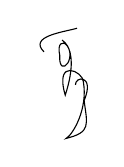
\begin{tikzpicture}[x=1cm,y=1cm]
\draw[thin] (0,1.1) .. controls (-.2,1.3) and (.25,1.35) .. (.42,1.4);
\draw[thin] (.23,1.25) .. controls (.48,1.06) and (.18,.72) .. (.2,1.06)
.. controls (.13,1.35) and (.5,1.25) .. (.27,.55)
.. controls (.13,1.03) and (.5,.85) .. (.5,.72)
.. controls (.56,.38) and (.37,.05) .. (.28,0)
.. controls (.6,.08) and (.55,.17) .. (.51,.48)
.. controls (.65,.82) and (.39,.79) .. (.4,.68);
\end{tikzpicture}
}
\margin{50}

\scanpage{52}
\margin{51}
\mspage{-3.18-}

form $\bar{\Phi}_0^{-1}(V)$ for some open neighborhood $V$ of $y$. Since $U_0$ is affine, it follows (for example, by SGA 8, Cor. 5.6) that $V$ is affine. Moreover, $U_0$ is defined by $P\ne0$, where $P$ is an invariant section of $(L_0\otimes\cdots\otimes L_m)^N$ (for suitable $N$). Then $P^{n+1}$ is induced by a section $s$ of $(M_0\otimes\cdots\otimes M_m)^N$ (cf. \S1), and $V$ must be defined by $s\ne0$. \uline{QED}

For the sake of the sequel, we fix a more explicit notation:
$(\mathbb{P}_n)_{\mathrm{stable}}^{m+1}$ instead of $U_{\mathrm{stable}}$, (cf. Proposition 7.7).

\scanpage{53}

\textcircled{$k$}\quad $H^*(X^k)$
\deleted{\uline{générateurs}}

\uline{générateurs}
\diagram{$
\begin{array}{lll}
\uline{\text{degré }\unsure{n|m}}:
&\text{les }k\text{ transformés de }
&\unsure{y|\eta}\otimes\underbrace{1\otimes\cdots\otimes1}_{k-1}
=\overline{\unsure{y|\eta}}\\
&\text{les }\binom{k}{2}\text{ transformés de }
&\unsure{\delta_1^*|\delta_1}\otimes\underbrace{1\otimes\cdots\otimes1}_{k-2}
=\bar\delta_1\\
\uline{\text{degré }2\unsure{n|m}}:
&\text{les }\binom{k}{3}\text{ transformés de }
&\delta_2\otimes\underbrace{1\otimes\cdots\otimes1}_{k-3}
=\bar\delta_2\\
\cdots&&\cdots\\
\uline{\text{degré }r\unsure{n|m}}:
&\text{les }\binom{k}{\unsure{r+1}}\text{ transformés de }
&\delta_r\otimes\underbrace{1\otimes\cdots\otimes1}_{k-1-r}
=\bar\delta_r\\
\cdots&\vdots&\cdots\\
\text{degré }(k-1)\unsure{n|m}:&\delta_{k-1}&=\bar\delta_{k-1}
\end{array}
$}

\deleted{\uline{relations}}

\uline{relations}
\margin{52}

\scanpage{54}
\margin{53}
\mspage{-3.17-}

section of $\{L_0\otimes\cdots\otimes L_m\}^M$ for some $M$, and such that $U_0\subset U_{\mathrm{stable}}$.
\deleted{\unsure{stable.}}

\uline{Proof}: Let $N\geq N_0>0$, and $P_0,\ldots,P_m$ be given by the Proposition. Moreover, let $P=P_0\otimes\cdots\otimes P_m$, and let $M=(m+1)N-N_0$. Then $P$ is a section of the ample invertible sheaf $(L_0\otimes\cdots\otimes L_m)^M$; hence $P\ne0$ defines an affine open neighborhood of $x$. Moreover, if $P(y)\ne0$ for some geometric point $y$ of $(\mathbb{P}_n)^{m+1}$, then $P_0(y)\ne0,\ldots,P_m(y)\ne0$, hence $y$ is stable by Proposition 3.6.
\uline{QED}

We can now apply our work to obtain the final result. Let $(Z,\unsure{\Phi|\bar\Phi})$ be the geometric quotient of $U_{\mathrm{reg}}$ by $\mathrm{PGL}(n)$. Let $Z_0\subset Z$ be the open subset such that $\unsure{\Phi|\bar\Phi}^{-1}(Z_0)=U_{\mathrm{stable}}$. Let $\unsure{\Phi|\bar\Phi}_0$ be the restriction of $\unsure{\Phi|\bar\Phi}$ to a morphism from $U_{\mathrm{stable}}$ to $Z_0$.

\uline{Theorem 3.8}: $(Z_0,\unsure{\Phi|\bar\Phi}_0)$ is a geometric quotient of $U_{\mathrm{stable}}$ by $\mathrm{PGL}(n)$, and, in fact, $U_{\mathrm{stable}}$ is a locally trivial principal fibre bundle over $Z_0$ with group $\mathrm{PGL}(n)$. Moreover, $M_0\otimes\cdots\otimes M_m$ is ample on $Z_0$, hence $Z_0$ is a quasi-projective scheme.

\uline{Proof}: The first part is clear. To prove the second part, it suffices to show that if $y$ is any geometric point of $Z_0$, then $y$ has an affine open neighborhood of the form $(Z_0)_s$ for some section $s$ of $(M_0\otimes\cdots\otimes M_m)^N$, (cf. EGA 2, Remark following Theorem 4.5.2). But let $x$ be a geometric point of $U_{\mathrm{stable}}$ over $y$. The open neighborhood $U_0$ of Corollary 3.7 is invariant, hence of the

\scanpage{55}
\diagram{\begin{tikzcd}[row sep=small]
X^{k-i}\arrow[r]&X^k\\
{}&{[1,k']\subset[1,k]}\arrow[l,"\text{surj}"']\\
&X^I
\end{tikzcd}}
\[
I=I'\amalg I''\qquad \text{Relation d'équivalence en }I'
\]
$I$ avec une division en un ens de parties
\deleted{non vides}, comprenant la partie vide
et le choix d'une de ses parties
\[
(R,J)\qquad
\left\{\begin{array}{l}
R\subset\unsure{\mathfrak P|\mathcal P}(I)\text{ tel que }\deleted{\unsure{\Longrightarrow}}
\left\{\begin{array}{ll}
a)&\displaystyle\coprod_{\unsure{J|A}\in R}A=I\\
b)&\unsure{A,A'\in R,\ A\ne A'\ \Longrightarrow\ A\cap A'=\varnothing}\\
c)&\varnothing\in R
\end{array}\right.\\[8pt]
J\in R
\end{array}\right.
\]
\[
\varepsilon_{R,J}\varepsilon_{R',J'}
=\left\{\begin{array}{ll}0&\text{si }J\cap J'\ne\varnothing\\[6pt]&\end{array}\right.
\]
\deleted{\unsure{\S}}
Supposons $J\cap J'=\varnothing$
\[
Z_{R,J}=\left\{(x_i)_{i\in I}\text{ tels que }
\left\{\begin{array}{ll}
x_i=a&\text{si }i\in J\\
x_i=x_j&\text{si }\exists A\in R,\text{ t.q. }i,j\in A
\end{array}\right.\right\}
\]
\[
Z^a_{R,J}\cap Z^{a'}_{R',J'}=Z_{R'',J''}
\]
\margin{du pt de vue ens.}
\margin{$R''$ est la relation d'équivalence \uline{engendrée} par $R,R'$.}
\[
\begin{array}{ll}
\widetilde J&\text{la classe }\deleted{\unsure{de J}}\inserted{\text{engendrée par}}\,J\\
\widetilde J'&\text{\unsure{---}}\ \deleted{\text{engendrée par}}\,J'
\end{array}
\]
\deleted{$\widetilde J\ne\widetilde J'$}
\[
\left\{\begin{array}{l}
\widetilde J=\widetilde J'\ne\varnothing
\quad\Longrightarrow\quad
\varepsilon_{R,J}\varepsilon_{R',J'}=0\\[8pt]
\widetilde J\ne\widetilde J'\ \text{ou }\widetilde J=\widetilde J'=\varnothing
\quad\text{alors}\quad
\varepsilon_{R,J}\varepsilon_{R',J'}
=\left(\displaystyle\prod_{i\in\widetilde J\cup\widetilde J'}\unsure{y|\eta}_i\right)
\displaystyle\prod_{\substack{A''\in R''\\A''\ne\widetilde J\\A''\ne\widetilde J'}}
\varepsilon_{\unsure{R_{A''}}}^{\deleted{\unsure{A''}}}
\varepsilon_{\unsure{R'_{A''}}}^{\deleted{\unsure{A''}}}
\end{array}\right.
\]
On est ramené au cas où $J=\varnothing$, $J'=\varnothing$,
et la relation d'équivalence \uline{engendrée} par $R,R'$ est la relation
\uline{grossière}.
Alors, \unsure{ensemblistement}, on obtient la diagonale de $X^I$
\margin{54}

\scanpage{56}
\mspage{-3.15-}
\margin{55}
suppose
\[
\begin{array}{rl}
\text{(i)}&x^{(0)}=x^{(1)}=\cdots=x^{(\beta_0)}\ne x^{(\beta_0+1)}\\[5pt]
\text{(ii)}&x^{(0)},x^{(1)},\ldots,x^{(\beta_1)}
\quad\text{all lie on exactly one line, but}\\
&x^{(\beta_1+1)}\quad\text{is not on this line.}\\[5pt]
\text{(iii)}&x^{(0)},x^{(1)},\ldots,x^{(\beta_2)}
\quad\text{all lie on exactly one plane, but}\\
&x^{(\beta_2+1)}\quad\text{is not in this plane,}\\
&\vdots\\
\text{(n)}&x^{(0)},\ldots,x^{(\beta_{n-1})}
\quad\text{all lie in exactly one hyperplane, but}\\
&x^{(\beta_{n-1}+1)}\quad\text{is not in this hyperplane.}
\end{array}
\]
Then $x^{(0)},x^{(\beta_0+1)},\ldots,x^{(\beta_{n-1}+1)}$
do not lie in a hyperplane, hence
$D_{0,\beta_0+1,\ldots,\beta_{n-1}+1}(x)\ne0$;
and whenever $D_{\alpha_0,\alpha_1,\ldots,\alpha_n}(x)\ne0$, then
\[
\alpha_0\ge0,\quad\alpha_1\ge\beta_0+1,\quad
\alpha_2\ge\beta_1+1,\ldots,\alpha_n\ge\beta_{n-1}+1.
\]
Therefore, the condition on $\ell$ is that:
\[
(*)\qquad\ell(d_{0,\beta_0+1,\ldots,\beta_{n-1}+1})\ge0.
\]
But it is easy to check that the set of all $\{\lambda\}$'s such that
$\lambda_0\le\cdots\le\lambda_m$
and $\displaystyle\sum_{i=0}^m\lambda_i=0$ is a convex set spanned by the particular set of
$\{\lambda\}$'s given in the lemma. Therefore $(*)$ holds for some $\ell$ if and only
if it holds for one of the extreme sets of $\{\lambda_i\}$.
\uline{QED}

Removing the assumption $\lambda_0\le\cdots\le\lambda_m$, and computing $\ell$ we
conclude that the existence of the P's is equivalent to:

\scanpage{57}
\[
\begin{array}{lll}
1\le\operatorname{card}R=s\le k&
\text{donc }\dim Z_R=\deleted{\unsure{n}}sn&
\operatorname{codim}Z_R=kn-sn=(k-s)n\\
\operatorname{card}R'=s'&&\operatorname{codim}Z_{R'}=(k-s')n\\
\operatorname{card}R''=1&&\operatorname{codim}Z_{R''}=(k-1)n
\end{array}
\]
\[
(k-1)n\le(k-s)n+(k-s')n
\quad\text{i.e.}\quad\deleted{\unsure{k\ge s+s'-1}}
\qquad\boxed{s+s'\le k+1}
\]
Cas d'égalité $\uline{s+s'=k+1}$ : on trouve la diagonale $\delta_k$.
\margin{\uline{! vérifier}\quad\uline{OK}}
Cas d'inégalité\quad
$k+1>s+s'$\quad i.e. $\unsure{k\ge s+s'}$
\deleted{donc il faut voir.}
\deleted{$\unsure{k\ge s+s'}$}
\[
\left|\begin{array}{ll}
1)&k>s+s'\quad\text{alors }\varepsilon_R\varepsilon_{R'}=0
\quad\text{pour raison de degrés}\\
2)&k=s+s',\quad\text{alors }\varepsilon_R\varepsilon_{R'}
=\underset{?}{\unsure{\chi}}\unsure{y|\eta}_{X^k}
\end{array}\right.
\]
\margin{\uline{! vérifier}}

\diagram{\begin{tikzcd}
X^s\arrow[r,hook]&X^k\\
&X^{s'}\arrow[u,hook]
\end{tikzcd}}
$s+s'=k\text{ ou }k+1$.

\deleted{$k\in\unsure{1+s+s'}$}
\diagram{\begin{tikzcd}
V^s\arrow[r]&V^k\\
V\arrow[u]\arrow[r]&V^{s'}\arrow[u]
\end{tikzcd}}

\diagram{\begin{tikzcd}
&U\arrow[dr,hook,no head,"p"]&\\
U\cap V\arrow[ur,hook,no head]\arrow[dr,hook,no head]&&W\\
p+q-r&V\arrow[ur,hook,no head,"q"']&
\end{tikzcd}}

\diagram{\begin{tikzcd}
&U'\arrow[dl,-,"\deleted{\unsure{p}}\ q-r"']\arrow[dr,-,"p-r"]&&\\
U'\cap V'\arrow[dr,-,"p-r"']&&U'+V'\arrow[r,-,"r"]&W'\\
&V'\arrow[ur,-,"q-r"']&&
\end{tikzcd}}
\margin{$\unsure{r}$}

a) Stable par $\boxtimes$ : clair

b) Stable par images inverses par projections
simpliciales : clair \deleted{$\unsure{\longrightarrow}$}

c) Stable par images \uline{directes} par projections

$i\in I$ et on prend projection
\[
X^I\mathbin{-}X^{I-\{i\}}
\]
a) $i\in J$ : clair

b) $i\notin J$ : on est ramené au cas de
\[
\delta_I\in H^*(X^I)\longrightarrow H^*(X^{I-\{i\}})
\qquad\text{on trouve }\unsure{\delta_{\bar I}|\delta_I}.
\]
\diagram{\begin{array}{ccc}
X^p&\longrightarrow&X^q\\
X^p\times X&-&X^q\times X\\
\Delta_p&-&\Delta_q\\
\Delta_{p\amalg1}&\longleftarrow&\Delta_{q\amalg1}
\end{array}}
\deleted{d) \unsure{Stable par images} \unsure{extraordinaires}
\unsure{contravariantes} des \unsure{diagonales}
\illegible{4}}

Stable par comp

\[
\boxed{\text{engendré, via }\boxtimes,\text{ par }\deleted{\unsure{\xi}},
\unsure{y|\eta},\text{ et les }\delta_I}
\]
\[
(\delta_{\unsure{1|2}}\boxtimes\delta_2)
\]
\margin{56}

\scanpage{58}
\mspage{-3.14-}
\margin{57}
\[
\begin{aligned}
(1,\ldots,1)\in\text{interior of }C_x
&\Longleftrightarrow
\begin{gathered}
\text{there are integers }N\ge N_0>0\\
\text{such that positive integral sums of}\\
\text{the d's generating }C_x\text{ are}\\
\text{the points:}\\
(N-N_0,N,\ldots,N),(N,N-N_0,\ldots,N),\\
\ldots,(N,N,\ldots,N-N_0)
\end{gathered}\\
&\Longleftrightarrow
P_i\text{, as in the Proposition, exist.}
\end{aligned}
\]
But on the other hand, $\{(1,1,\ldots,1)\notin\text{ interior of }C_x\}$ is
equivalent to the existence of a linear functional $\ell$ on E such that
$\ell((1,1,\ldots,1))=0$, and $\ell(d_{\alpha_0,\ldots,\alpha_n})\ge0$ for every d
generating $C_x$. Suppose
\[
\ell((z_0,\ldots,z_m))=\sum_{i=0}^m\lambda_i z_i.
\]
Without loss of generality, we may assume that $\lambda_0\le\lambda_1\le\cdots\le\lambda_m$.
The key point is:

\uline{lemma}: If for some set of $\lambda_i$ such that $\lambda_0\le\lambda_1\le\cdots\le\lambda_m$
and $\displaystyle\sum_{i=0}^m\lambda_i=0$, then
$\ell(d_{\alpha_0,\ldots,\alpha_n})\ge0$ for every $d_{\alpha_0,\ldots,\alpha_n}$
generating $C_x$, then, in fact, this happens for some $\{\lambda_i\}$ of the form:
\[
\lambda_0=\lambda_1=\cdots=\lambda_\beta=-(m-\beta)
\]
\[
\lambda_{\beta+1}=\cdots=\lambda_m=+(\beta+1).
\]
\uline{Proof}: The point is that if $\lambda_0\le\cdots\le\lambda_m$, then we can pick,
\uline{a priori}, that determinant $D_{\alpha_0,\ldots,\alpha_n}$ which is not zero at x, and
for which $\ell(d_{\alpha_0,\ldots,\alpha_n})=\displaystyle\sum_{i=0}^n\lambda_{\alpha_i}$
assumes its minimum value. Namely,

\cotefile{56}
\scanpage{2}
\margin{\unsure{3 p|30}}
Situation des

``vanishing cycles'' ;

\unsure{irréductibilité}

Cas des Quadriques
\margin{1}

\scanpage{3}
\margin{\figure{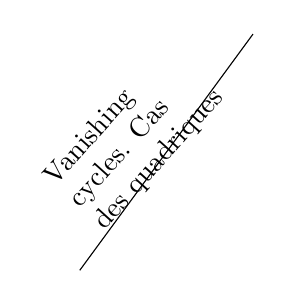
\begin{tikzpicture}[baseline]
\draw (0,0)--(2.2,3);
\node[rotate=48,anchor=west,align=left] at(-.15,.75)
{\uline{Vanishing}\\cycles. Cas\\des quadriques};
\end{tikzpicture}}}
\diagram{\begin{tikzcd}X\arrow[d,"f"]\\S\end{tikzcd}}
$f$ morphisme projectif plat

$S$ spectre d'un anneau de val discrète strictement local

$X_0$ fibre spéciale quadrique à point singulier

$\bar X_1$ fibre géom générique, quadrique non singulière

dimension commune des fibres $n-1$

\unsure{\big[}
\deleted{\unsure{On veut étudier}}
$X\deleted{\unsure{n}}\subset\mathbf P^n_S$ défini par une équation quadratique \ldots

\[
H^i(X_0)\mathbin{-}H^i(\bar X_1)\qquad ?
\]
On a la suite exacte générale
\[
\cdots\mathbin{-}H^i(X_0)\mathbin{-}H^i(\bar X_1)
\mathbin{-}\Phi^{i+1}\mathbin{-}H^{i+1}(X_0)
\mathbin{-}H^{i+1}(\bar X_1)\mathbin{-}\cdots
\]
On sait que la cohomologie de \deleted{$H^*(X_0)$ et}
\deleted{1°) \uline{$n$ pair}, \unsure{donc $n-1$ impair}}
$X_0$ et $\bar X_1$ est nulle en dim impaires. Donc
on trouve
\[
0\longrightarrow\Phi^{2\nu}\longrightarrow H^{2\nu}(X_0)
\mathbin{-}H^{2\nu}(\bar X_1)\longrightarrow\Phi^{2\nu+1}\mathbin{-}0
\]
i.e. les $\Phi^i$ apparaissent exactement comme les
noyaux et conoyaux du \uline{hom. de spécialisation}.

Notons aussi que sur $X$ donc $X_0$, on a une
classe $\xi\in H^2(X,\unsure{\mu}(1))$, provenant de la section
à l'infini, et dont la restriction à chaque fibre
est connue \ldots
\margin{2}

\scanpage{4}
\mspage{\unsure{63|68}}
\deleted{
a) La fonction $\rho_r$ sur S est semi-continue inférieurement, la
fonction $\rho_n$ sur S est semi-continue supérieurement, donc la fonction
$\rho_u=\rho_n-\rho_r$ est semi-continue supérieurement.

b) Les \deleted{\unsure{c}}conditions suivantes (stables par changement de base
quelconque) sont équivalentes:

(i) La fonction $\rho_r$ sur S est localement constante.

(ii) Il existe localement, au sens de la topologie étale,
un tore maximal dans G.

(ii bis) Il existe localement, au sens de la topologie
fidèlement plate quasi-compacte, un tore maximal dans G.

c) Soient $T_1,T_2$ deux tores maximaux dans G (ce qui implique que
l'on est sous les conditions envisagées dans b). Alors $T_1,T_2$ sont
\figure{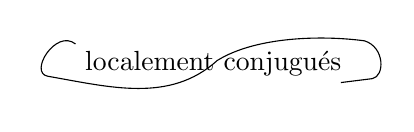
\begin{tikzpicture}[baseline=(t.base)]
\node[inner sep=2pt] (t) {localement conjugués};
\draw (-1.75,.25) .. controls (-2,.45) and (-2.35,-.12) .. (-2.1,-.16)
.. controls (-1.3,-.3) and (-.55,-.5) .. (.05,.04)
.. controls (.55,.35) and (1.4,.36) .. (1.92,.29)
.. controls (2.18,.21) and (2.18,-.16) .. (2.02,-.19)
--(1.62,-.24);
\end{tikzpicture}}
au sens de la topologie étale, i.e. il existe
un morphisme étale surjectif $S'\to S$ tel que les sous-groupes $T_{1\,S'}$ et
$T_{2\,S'}$ de $G_{S'}$ soient conjugués par une section de $G_{S'}$ sur $S'$.

d) Sous les conditions de b), i.e. lorsque $\rho_r$ est localement
constante, il en est de même de $\rho_n$ (donc aussi de $\rho_u=\rho_n-\rho_r$).

Démonstration.

a) Notons que pour tout morphisme $S'\to S$, si $G'=G\times_S S'$, les
fonctions $\rho'_r$ etc sur $S'$ \deleted{construites à l'aide} définies en termes de
G' comme $\rho_r$ etc en termes de G, s'obtiennent simplement \deleted{comme} en composant
ces dernières avec $S'\to S$. Lorsque $S'\to S$ est fidèlement plat quasi
compact, il en résulte que $\rho'$ est continue, resp. semi-continue
supérieurement, resp. semi-continue inférieurement, si et seulement si
$\rho$ l'est, \deleted{(SGA VIII} la topologie \inserted{de Zariski} de S étant en effet quotient de celle
de S' (SGA VIII 4.3.). Par suite, les assertions de a) sont locales pour
}
\margin{3}

\scanpage{5}
1°) \uline{$n$ pair}$=2\nu$,\quad \uline{$n-1$ impair}
\qquad $n-1=2\nu-1=2(\nu-1)+1$
\diagram{\[
\left.\begin{array}{ll}
H^*(X_0):&
1,\xi_0,\ldots,\xi_0^{\nu-1},
[\xi_0^\nu,\lambda'_\nu],\frac12\xi_0^{\nu+1},\ldots,\frac12\xi_0^{2\nu-1}\\[5pt]
H^*(\bar X_1):&
1,\xi_1,\ldots,\xi_1^{\nu-1},
\frac12\xi_1^\nu,\frac12\unsure{\xi_1^{\nu+1}},\ldots,\frac12\xi_1^{2\nu-1}
\end{array}\right]
\quad
\begin{array}{l}\xi_0\rightsquigarrow\xi_1\\\lambda'_\nu\rightsquigarrow0\end{array}
\]}
Donc\quad $H^i(X_0)\mathbin{-}H^i(\bar X_1)$
\uline{bijectif} \deleted{excepté} si $i\ne2\nu=n$

$H^{2\nu}(X_0)\mathbin{-}H^{2\nu}(\bar X_1)$
\uline{surjectif}, noyau engendré par $\lambda'_\nu$.
\[
\text{Donc}\qquad
a)\left\{\begin{array}{ll}
\Phi^i=0&\deleted{\text{sauf}}\ \text{si }i\ne(2\nu=n)\\
\Phi^{\unsure{2\nu|n}}\simeq\unsure{\mu|M}(-\nu)&
\text{(isom. déterminé au signe près\ldots)}
\end{array}\right.
\]
\[
b)\left\{\begin{array}{l}
R^if_*\text{ constant si }i\ne n\\
R^nf_*\text{ a un sous-faisceau concentré en o, isom. à }\unsure{\mu|M}(\ldots),\\
\text{le quotient par ce dernier est constant}
\end{array}\right.
\]
\margin{c) $\pi$ opère trivialement sur $H^*(\bar X_1)$ et sur $\Phi^{2\nu}$}

\figure{\begin{tikzpicture}
\draw (0,0)--(8,.3) .. controls (8.3,.3) and (8.1,-.4) .. (8.4,-.5)--(10.4,-.5);
\end{tikzpicture}}
2°) $n$ impair $=2\nu+1$,\qquad $n-1=2\nu$
\diagram{\[
\left.\begin{array}{ll}
H^*(X_0):&
1,\xi_0,\ \xi_0^{\nu-1},\ \xi_0^\nu,\ \frac12\xi_0^{\nu+1},
\ldots,\frac12\xi_0^{2\nu}\\[5pt]
H^*(\bar X_1):&
1,\xi_1,\ldots,\xi_1^{\nu-1},[\xi_1^\nu,\lambda_\nu],
\frac12\xi_1^{\nu+1},\ldots,\frac12\xi_1^{2\nu}
\end{array}\right]
\quad\xi_0\rightsquigarrow\xi_1
\]}
Donc\quad $H^i(X_0)\mathbin{-}H^i(\bar X_1)$ bijectif si $i\ne2\nu=n-1$

$H^{2\nu}(X_0)\mathbin{-}H^{2\nu}(\bar X_1)$ injectif,
conoyau engendré par $\deleted{\unsure{\xi}}\unsure{\lambda_\nu}$.
\[
a)\left\{\begin{array}{ll}
\Phi^i=0&\text{si }i\ne2\nu+1=n\\
\Phi^n\simeq\unsure{\mu|M}(\unsure{?}\ldots)&
\end{array}\right.
\]
\[
b)\left\{\begin{array}{l}
R^if_*\text{ constant si }i\ne n-1\\
R^{n-1}f_*\text{ est ``pur''}\ldots
\end{array}\right.
\]
\margin{c) $\pi$ opère trivialement sur les $H^i(\bar X_1)$ pour $i\ne n-1$,
mais non sur $\Phi^n$ \ldots}
\margin{4}

\scanpage{6}
\mspage{1}
\margin{\deleted{\unsure{II}}}
\deleted{
1. \uline{Tores maximaux.}\deleted{\unsure{et centralisateurs}}

\deleted{A partir de maintenant, nous ferons usage des résultats du
Séminaire Chevalley 56/57 sur les Groupes Algébriques. Suivant l'usage
en théorie des groupes algébriques, nous référons à ce Séminaire par le
sigle BIBLE.}

Soit d'abord G un groupe algébrique sur un corps \uline{algébriquement
clos} k. On appelle \uline{tore maximal} de G un \deleted{tore} sous-groupe algébrique
T de G qui est un \uline{tore} (ce qui signifie ici, k étant algébriquement
clos, qu'il est isomorphe à un groupe de la forme $G_m^r$), et qui est
maximal pour cette propriété. Noter que, k étant parfait, $G_{\mathrm{réd}}$ est
un sous-groupe de G, lisse sur k, c'est donc essentiellement un groupe
algébrique au sens de BIBLE. D'ailleurs, tout sous-groupe réduit de G
(tel un tore) est automatiquement un sous-groupe de $\unsure{R|G}_{\mathrm{réd}}$, par suite les
tores maximaux de G coïncident avec les tores maximaux de $G_{\mathrm{réd}}$. Lorsque
G est affine, donc $G_{\mathrm{réd}}$ affine, un théorème fondamental de Borel
nous dit que deux tores maximaux de G sont conjugués \deleted{\illegible{1}} par un
élément de $G(k)$ \inserted{$=G_{\mathrm{réd}}(k)$} (BIBLE 6, th.4 c ), en particulier ils ont même
dimension. \inserted{Nous appellerons} \deleted{L}\inserted{l}a dimension commune des tores maximaux de G \deleted{est alors appelée}
le \uline{rang réductif} de G. Noter d'ailleurs que la restriction G affine
est inutile, comme il résulte d'un théorème \deleted{\unsure{bien}} connu de Chevalley,
affirmant que tout groupe algébrique connexe lisse sur k est une
extension d'une variété abélienne par un groupe affine\deleted{\unsure{un}};
\deleted{nous n'aurons
pas besoin de cette généralisation.}\inserted{cf N°6 $\unsure{\xi|\S}$.}

Dans \inserted{les N°s 1 à 4,} nous nous bornerons \deleted{aux groupes algébriques}
\inserted{le plus souvent aux} préschémas
en groupes affines sur la base.
\deleted{G sur k étant comme ci-dessus,}
\inserted{Soit G un groupe algébrique lisse sur k,} et T
un tore maximal de G, le centralisateur \inserted{$C(T)$} de T dans G sera appelé le
}
\margin{\figure{\begin{tikzpicture}[baseline=(t.base)]
\node[draw,circle,inner sep=5pt] (t) {$G_{\mathrm{réd}}(k)$};\end{tikzpicture}}}
\margin{pas à la ligne}
\margin{à la ligne \figure{\begin{tikzpicture}[baseline]
\draw (0,0)--(.4,0)--(.4,.3)--(.9,.3);\end{tikzpicture}}}
\margin{5}

\scanpage{7}
\uline{Calculs Affines}\qquad
Nous remplaçons $X$ par $U=X-\unsure{Z}$

(\deleted{section} à l'infini), on aura
\[
\cdots\longrightarrow H^i(U_0)\mathbin{-}H^i(\bar U_1)
\mathbin{-}\Phi^{i+1}\mathbin{-}H^{i+1}(X_0)
\mathbin{-}H^{i+1}(\bar X_1)\mathbin{-}\cdots
\]
Or on a maintenant \uline{$H^i(U_0)=0$}\qquad $i\ne0$,
\[
\text{d'où}\qquad H^i(\bar U_1)\simeq\Phi^{i+1}
\]
d'où directement
\[
\Phi^i=0\quad\text{si }i\ne n
\]
\[
\Phi^n=H^{n-1}(\bar U_1)
\quad\text{engendré par les ``vanishing cycles''}\ldots
\]
\margin{6}

\scanpage{8}
\mspage{0}
XII\quad \uline{Tores maximaux}, \uline{groupe de Weyl}, \uline{sous-groupes de Cartan}, \uline{centre
réductif des schémas en groupes lisses et affines}.

par A. Grothendieck.

A partir du présent exposé, contrairement aux exposés précédents,
nous ferons usage des résultats connus sur la structure des groupes
algébriques lisses sur un corps algébriquement clos k, et surtout
de la théorie de BOREL des groupes algébriques affines, exposée dans
le Séminaire CHEVALLEY 56/57: \deleted{sur les Groupes} ``Classification des
groupes de Lie Algébriques''. Suivant l'usage en théorie des groupes
algébriques, nous référons à ce Séminaire par le sigle BIBLE. Pour les
\deleted{moment,}\inserted{prochains exposés,} nous aurons besoin \inserted{notamment} des résultats de\deleted{s} BIBLE 4, 5, 6, 7
(le chiffre après BIBLE renvoie au numéro de l'exposé). Il \deleted{\unsure{me}} semble
\deleted{\illegible{1}}\inserted{d'ailleurs} que la théorie des schémas \inserted{n'}apporte aucune simplification notable
à la théorie \deleted{exposée} de BOREL \deleted{\unsure{en question}} telle qu'elle est exposée
dans BIBLE. C'est pourquoi il n'a pas semblé utile de la reproduire \deleted{ici}
\deleted{notre objet étant} dans le présent Séminaire, notre but étant ici de
déduire, de résultats connus sur les corps algébriquement clos, des
résultats analogues valables sur tout préschéma de base. (Il n'en sera
plus de même pour la théorie de structure de CHEVALLEY des groupes
semi-simples, qui, semble-t-il, se traite avec avantage ab ovo sur un
préschéma de base quelconque).

\inserted{Dans les exposés oraux \inserted{\figure{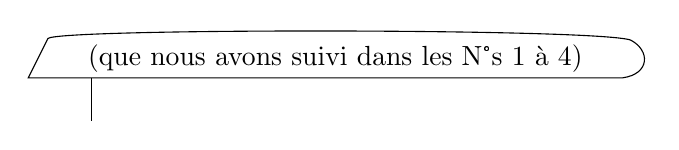
\begin{tikzpicture}[baseline=(t.base)]
\node[inner sep=3pt] (t) {(que nous avons suivi dans les N°s 1 à 4)};
\draw (-3.9,-.25)--(-3.65,.25) .. controls (-3.5,.38) and (3.3,.38) .. (3.75,.23)
.. controls (4,.1) and (4,-.2) .. (3.65,-.25)--cycle;
\draw (-3.1,-.25)--(-3.1,-.8);
\end{tikzpicture}}}
nous nous étions limités aux
préschémas en groupes affines sur S, en nous appuyant
de façon essentielle sur les théorèmes de représentabilité
de Exp $\overline{\underline{\mathrm{XI}}}$ N°4. Dans les présentes notes (cf
N°s 6 à \unsure{8}) nous montrons rapidement comment on peut
éliminer les hypothèses affines \deleted{\unsure{par une méthode plus}}
\inserted{par une \deleted{\illegible{1}} méthode} plus
simple n'utilisant pas les résultats les plus délicats de Exp. $\overline{\underline{\mathrm{XI}}}$.}
\figure{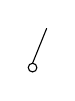
\begin{tikzpicture}[baseline]\draw (0,0) circle (.055);\draw (0,.055)--(.18,.5);\end{tikzpicture}}

\margin{Pour d'autres généralisations des résultats contenus
dans le présent exposé, voir également exposés
\deleted{\unsure{Exp.}}$\overline{\underline{\mathrm{XV}}}$ et $\overline{\underline{\mathrm{XVI}}}$. (Il est évident que le contenu des
exposés $\overline{\underline{\mathrm{XI}}}$, $\overline{\underline{\mathrm{XII}}}$, $\overline{\underline{\mathrm{XV}}}$, $\overline{\underline{\mathrm{XVI}}}$ devrait être complètement refondu).}
\margin{\figure{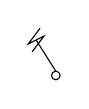
\begin{tikzpicture}[baseline]\draw (0,0) circle (.055);\draw (0,.055)--(-.25,.45);\draw (-.3,.3)--(-.15,.5)--(-.35,.4)--(-.2,.6);\end{tikzpicture}}}
\margin{7}

\scanpage{9}
\margin{\unsure{12 p}}
Calculs de cohomologie

des quadriques,

des cônes projetants
\margin{8}

\scanpage{11}
\uline{Cohomologie d'un cône projectif}.
\diagram{\begin{tikzcd}
X\arrow[d,"h"]&&\\
C'\arrow[d]\arrow[r,hook,no head,"i'"]&
\hat C'\arrow[d]\arrow[r,bend left=30]&X'\arrow[l,hook',"j'"']\arrow[d,"\simeq"]\\
C\arrow[r,hook,"i"]\arrow[rr,bend right=30]&
\hat C&X\arrow[l,hook',"j"']
\end{tikzcd}}
\margin{\deleted{$\unsure{\sim}$}}
\[
E=C-a\qquad \hat E=\hat C-a
\]
\margin{$i>0$}
\deleted{$H^{i-1}(X)\to H^i(\hat C)\to H^i(\hat C')\to H^i(X)\to H^{i+1}(\hat C)$}
\deleted{$H^i(C)$}
\diagram{\begin{tikzcd}[column sep=small]
\cdots\arrow[r,-,"\text{surj}"]&
H^{i-1}(X)\arrow[r,-]\arrow[d,-]&
H^i(\hat C)\arrow[r,-]\arrow[d,-]&
H^i(\hat C')\arrow[r,-,"\text{surj}"]\arrow[d]&
H^i(X)\arrow[r,-]\arrow[d,-]&\cdots\\
&H^{i-1}(X)\arrow[r,-]&H^i(C)\arrow[r,-]&H^i(C')\arrow[r,-,"\text{bij}"]&H^i(X)&
\end{tikzcd}}
\[
\boxed{H^i(C)=0\qquad i\ne0}
\]
\[
0\longrightarrow H^i(\hat C)\longrightarrow H^i(\hat C')
\longrightarrow H^i(X)\longrightarrow0
\]
\[
\boxed{H^i(\hat C)\xleftarrow{\sim}H^{i-2}(X)(-1)\qquad i\ne0}
\]
provenant de l'injection
\[
X\xrightarrow{j}\hat C
\]
\[
j_*(a)j_*(b)=j_*(ab\xi)\qquad\text{car }j^*j_*(c)=c\xi,
\]
cela détermine la structure multiplicative \ldots

$\unsure{*}\ \begin{array}{c}\hat C-a\\[-3pt]\rotatebox{90}{$\simeq$}\\[-3pt]\hat C'-a\end{array}$
est fibré sur $X$ \unsure{de fibres des droites}
\deleted{affi-}\inserted{vectorielles},
donc
\[
\boxed{H^*(X)\xrightarrow{\sim}H^*(X,\underbrace{\hat C-a}_{\hat E})}
\]
\[
\hat C-a=\hat E\qquad \hat C-a-X=E
\]
\diagram{\begin{tikzcd}[column sep=small]
H^{i-2}(X)(-1)\arrow[r,"\text{multiplicat. par }\xi\text{ (ou }-\xi\text{)}"']&
H^i(\hat E)\arrow[r]\arrow[d,-,"\simeq"]&
\boxed{H^i(E)}\arrow[r]&
H^{i-1}(X)(-1)\arrow[r]&H^{i+1}(\hat E)\arrow[d,-,"\simeq"]\\
&H^i(X)&&&H^{i+1}(X)
\end{tikzcd}}
\margin{\deleted{$\unsure{\simeq}$}\quad\deleted{$\unsure{\simeq}$}}
\margin{10}

\scanpage{12}
\uline{Remarques} 1.11. a) Le préschéma $\unsure{\mathcal T|\tau}$ de 6.10. s'appellera comme de juste le
\uline{préschéma des tores maximaux} de G. On verra au N°5 qu'il est en fait \uline{affine}
sur S. On peut le vérifier directement, lorsque G est isomorphe à un
sous-préschéma en groupes fermé d'un préschéma de la forme $\mathrm{Gl}(n)$, en
utilisant Exp XI 4.6. et en remarquant que par le raisonnement de la
démonstration de 1.7. b), $\unsure{\mathcal T|\tau}$ s'identifie à un sous-préschéma à la fois
\uline{ouvert et fermé} du préschéma F qui représente les sous-groupes de type
multiplicatif de G.

b) Il \deleted{ne serait pas difficile}\inserted{est possible} de donner une démonstration de 1.7.
donc de 1.9, n'utilisant pas les résultats délicats de Exp XI, mais
seulement \inserted{les \deleted{\unsure{anciens}} résultats faciles} Exp XI 3.12.
\deleted{\unsure{de Exp XI N°6}}\inserted{et 6.2.}
en travaillant uniquement avec des groupes
de type multiplicatif finis sur la base (moralement, les groupes $\,{}_nT$ où T
est un tore maximal), comparer \deleted{\unsure{au}} N°7.
\deleted{Par contre,}\inserted{La même remarque vaut pour} la démonstration
de 1.10.
\deleted{s'appuie de façon essentielle sur Exp XI 4.\unsure{1}.
Dans un autre
exposé, nous donnerons une version généralisée de 1.10. par une démonstration
différente (s'appuyant sur un théorème de représentabilité de EGA \unsure{V|VI}).
\deleted{Exception faite \unsure{du Exp N°5},}
\inserted{De façon générale,}\inserted{pour les résultats du N°5,}
les théorèmes de représentabilité de Exp XI
N°4 \deleted{\unsure{vraisemblablement}} pourraient\deleted{\unsure{tous}}
être éliminés de la théorie
présentée \inserted{dans le présent exposé et les suivants}.}
\deleted{\inserted{de façon générale,
il est possible (et sans doute avantageux) d'éliminer
totalement les résultats de représentabilité de
Exp $\overline{\underline{\mathrm{XI}}}$ N°4 de la théorie présentée dans le
présent exposé et les suivants.}}
\margin{\figure{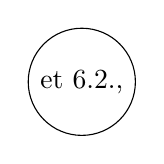
\begin{tikzpicture}[baseline=(t.base)]
\node[draw,circle,inner sep=3pt] (t) {et 6.2.,};\end{tikzpicture}}}
\margin{11}

\scanpage{13}
Si $X$ est non singulier \inserted{connexe de dim $n$}, on trouve
\[
\boxed{\begin{array}{lll}
i\le n&H^i(E)\simeq P^i(X)&\text{mod torsion}\\
i\ge n+1&H^i(E)\simeq\unsure{R|P}^{i-1}(X)(-1)&\text{mod torsion}
\end{array}}
\]
\margin{\unsure{Les versions du} th. de Lefschetz}
\[
\cdots\mathbin{-}
\underset{\substack{\Vert\\0\\\text{si }i-1\ne0}}{H^{i-1}(C)}
\mathbin{-}H^{i-1}(E)\mathbin{-}H^i_{\unsure{x|a}}(C)
\longrightarrow
\underset{\substack{\Vert\\0\\\text{si }i\ne0}}{H^i(C)}
\mathbin{-}H^i(E)\mathbin{-}H^{i+1}_{\unsure{x|a}}(C)\mathbin{-}\cdots
\]
\margin{$\unsure{A}$}
\deleted{$i\ne0,1$}
\[
\cdots\mathbin{-}\underset{\substack{\Vert\\0}}{H^0_{\unsure{x|a}}(C)}
\mathbin{-}H^0(C)
\xrightarrow[\uline{\text{si }X\text{ connexe}}]{\text{bij}}
H^0(E)\mathbin{-}H^1_{\unsure{x|a}}(C)
\longrightarrow\underset{\substack{\Vert\\0}}{H^1(C)}
\longrightarrow H^1(E)\mathbin{-}H^2_{\unsure{x|a}}(C)
\mathbin{-}\underset{\substack{\Vert\\0}}{\unsure{H^2(C)}}
\]
\figure{\begin{tikzpicture}[baseline]\draw[->] (0,0)--(.5,.45);\end{tikzpicture}}
\[
\boxed{\begin{array}{l}
H^0_{\unsure{x|a}}(C)=H^1_{\unsure{x|a}}(C)=0\\
H^i_{\unsure{x|a}}(C)\simeq H^{i-1}(E)\qquad\text{si }i\ge2
\end{array}}
\]
\figure{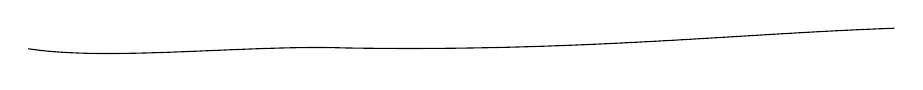
\begin{tikzpicture}\draw (0,.04) .. controls (1,-.12) and (2.8,.09) .. (4,.05) .. controls (7,.0) and (9,.23) .. (11,.3);\end{tikzpicture}}
Cas $X$ une quadrique $Q^n$, donc $\hat C=Q'^{n+1}$, on trouve
\[
\uline{H^i(Q'^{n+1})\xleftarrow{\sim}H^{i-2}(Q^n)(-1)}
\quad\text{si }i\ne0\qquad\text{donc:}
\]
\diagram{\[
\left|\begin{array}{ll}
\left(1,\xi,\ldots,\xi^\nu,\frac12\xi^{\nu+1},\ldots,\frac12\xi^{2\nu}\right)
&\text{si }\boxed{n+1=2\nu}\\[6pt]
\left(1,\xi,\ldots,\xi^\nu,[\xi^{\nu+1},\lambda'_{\nu+1}],
\frac12\xi^{\nu+2},\ldots,\frac12\xi^{2\nu+1}\right)
&\text{si }\boxed{n+1=2\nu+1}
\end{array}\right.
\]}
avec $\left\{\begin{array}{l}\xi\lambda'_{\nu+1}=0\\{\lambda'_{\nu+1}}^2=0\end{array}\right.$
\margin{12}

\scanpage{14}
\mspage{\unsure{84|82}}
dans G. Si C est son centralisateur, alors C est représentable et est
lisse sur S par \inserted{Exp $\overline{\underline{\mathrm{XI}}}$} 5.3., donc la fonction
$s\rightsquigarrow\rho_n(s)=\dim C_s$ est bien
localement constante.

\deleted{Corollaire}
La démonstration de 1.7. est achevée. Nous référerons aux
condition envisagées dans 1.7. b) en disant que dans ce cas, G est
de \uline{rang réductif localement constant}.\deleted{sur S} Notons:

\uline{Corollaire} 1.9. Soit G comme dans 1.7., et soit $s\in S$ tel que
\inserted{$\rho_u(s)=0$ i.e.}
$\rho_r(s)=\rho_{\unsure{m|n}}(s)$, (i.e. les sous-groupes de Cartan de $G_k$ sont des tores, où k
est une clôture algébrique de $k(s)$). Alors il existe un voisinage \deleted{ouvert}
ouvert U de S sur lequel $\rho_r$ et $\rho_n$ sont constants, en particulier pour
tout $t\in U$, le rang unipotent $\rho_u(t)$ de $G_t$ est nul.

En effet, \deleted{\unsure{l'hypothèse s'écrit aussi} $\rho_u(s)=0$, et comme} cela
résulte immédiatement de 1.7. a) et de l'inégalité $\rho_r(t)\le\rho_{\unsure{m|n}}(t)$ pour
tout $t\in S$.

Notons aussi que nous avons prouvé, en même temps que b), le

\uline{Corollaire} 1.10. Soit G comme dans 1.7., et supposons G de rang
réductif localement constant. Considérons le foncteur
\[
\unsure{\mathcal T|\tau}:(\mathrm{Sch})^o\longrightarrow(\mathrm{Ens}),
\]
tel que pour tout S' sur S, on ait
\[
\unsure{\mathcal T|\tau}(S')=\text{ensemble des tores maximaux de }G_{S'}.
\]
Alors $\unsure{\mathcal T|\tau}$ est représentable par un préschéma lisse, séparé et de
type fini sur S.

Il reste à vérifier que $\unsure{\mathcal T|\tau}$ est \deleted{\unsure{séparé}} de type fini sur S\unsure{!|?} La
question étant locale pour la topologie fidèlement plate quasi-compacte,
on peut supposer que G admet un tore maximal T. Mais alors $\unsure{\mathcal T|\tau}$
\deleted{\illegible{1}} est
\deleted{\illegible{1}}\inserted{isomorphe à}
$(G/\uline{\operatorname{Norm}}_G(T)$ (comparer \inserted{Exp $\overline{\underline{\mathrm{XI}}}$} 5.3. bis et 5.5.).
\deleted{\unsure{donc}} Le morphisme
$G\longrightarrow\unsure{\mathcal T|\tau}$ défini par $g\rightsquigarrow\operatorname{int}(g)(T)$ étant surjectif,
et G quasi-compact
sur S, il en est de même de $\unsure{\mathcal T|\tau}$, ce qui achève la démonstration.
\margin{13}

\scanpage{15}
\deleted{\diagram{\begin{tikzcd} &\unsure{A^+}\\ \unsure{A}\arrow[ur]&\end{tikzcd}}}
\[
\left\{\begin{array}{l}
\left.\begin{array}{l}
H^i(E)=0\quad
\deleted{\unsure{\xi}}\ \deleted{\text{si }i\ne\unsure{2(\nu-1)}}
\inserted{i\ne0,2\nu-2,4\nu-1}\\
H^{2(\nu-1)}(E)\simeq
\left\{\begin{array}{ll}0,&\ell\ne2\\
\mathbb Z/2\mathbb Z&\text{si }\ell=2
\end{array}\right.
\end{array}\right\}\\
H^{4\nu-1}(E)\simeq\unsure{\mu|M}(-2\nu)
\end{array}\right.
\qquad
\begin{array}{c}\boxed{n+1=2\nu}\\n=2\nu-1\end{array}
\]
\[
\left\{\begin{array}{l}
H^i(E)=0\quad\text{si }i\ne\inserted{0,}2\nu-1,2\nu+1,4\nu+1\\
H^0(E)=\unsure{\mu|M}(0)\\
H^{\unsure{2\nu-1}}(E)\simeq\unsure{\mu|M}(-\nu+1)\\
H^{\unsure{2\nu+1}}(E)\simeq\unsure{\mu|M}(-\nu-1)\\
H^{4\nu+1}(E)\simeq\unsure{\mu|M}(-2\nu-1)
\end{array}\right.
\qquad
\begin{array}{c}\boxed{n+1=2\nu+1}\\n=2\nu\end{array}
\]
\margin{14}

\scanpage{16}
\mspage{\unsure{160|16a}}

algébriquement clos. Mais alors, $s$ désignant le point fermé de $S$, comme $G$ est étale et séparé sur $S$, il contient un sous-schéma à la fois ouvert et fermé $G'$, \inserted{fini sur $S$,} tel que $G'_s=G_s$ \inserted{(EGA II 6.2.6.)}, et on voit de suite que $G'$ est ici un sous-groupe de $G$. \deleted{\unsure{Par suite la fibre géométrique $f(s)$}} D'ailleurs $G'$ \deleted{qui} étant étale fini sur $S$ \deleted{qui} $=\operatorname{Spec}(V)$, $V$ complet à corps résiduel algébriquement clos, est un groupe constant, donc de la forme $A_S$, où $A=G'(k(s))=G(k(s))$ a pour classe $f(s)$. \deleted{On voit donc} Si $B$ est la fibre géométrique de $G$ en le point générique $t$ de $S$, on a donc un \deleted{\unsure{homomor}}\inserted{monomor}phisme canonique $A\longrightarrow B$, ce qui prouve $f(s)\leq f(t)$. (NB cette démonstration prouve en fait la semi-continuité pour une relation d'ordre sur $E$ plus fine que celle indiquée dans 2.1.). Le fait que $f$ soit continue en $s$ si et seulement si $s\rightsquigarrow\operatorname{card}f(s)$ l'est résulte du fait que pour $w,w'\in E$, les relations \deleted{\unsure{w}} $w\leq w'$ et $\operatorname{card}w=\operatorname{card}w'$ impliquent $w=w'$. Le fait que cette condition soit équivalente à \deleted{\unsure{à}} la finitude de $W$ sur un voisinage de $s$ est alors indépendant de\deleted{s}\inserted{la} structure\deleted{s} de groupe\deleted{s}\inserted{sur $W$}, et a été signalé après \inserted{Exp $\overline{\underline{\mathrm{XI}}}$} 5.10. ; d'ailleurs sa démonstration \deleted{qui} se fait aisément par les arguments précédents, \inserted{en} utilisant le critère valuatif de propreté EGA II 7.3.8.

\uline{Lemme} 2.3. Soient $G$ un groupe algébrique affine lisse sur un corps algébriquement clos $k$, $R\subset T$ deux sous-tores, $W(R)$ et $W(T)$ les deux groupes finis associés comme dans \inserted{Exp $\overline{\underline{\mathrm{XI}}}$} 5.9., quotients du normalisateur par le centralisateur. Alors $W(R)$ est isomorphe à un quotient d'un sous-groupe de $W(T)$.

\deleted{Dans la démonstration qui suit, il sera commode d'interpréter $G$, $R,T$, $C(R),N(R)$, $C(T)$, $N(T)$ de façon purement ensembliste, comme les groupes de points des préschémas $G,R,T$ dans $k$, et les centralisateurs et nor}

\mspage{15}

\scanpage{17}
\uline{Cohomologie à supports compacts} \deleted{de} de $C,E,\widehat E\ldots$

Les \unsure{cohomologies} à support compact de $E,\widehat E$ se \unsure{déduit} simplement par dualité des \deleted{celles}\inserted{la coh. usuelle} de $E,\widehat E$ lorsque $X$ est lisse \unsure{\ldots\ (\ldots}. Celle de $\widehat C$ est identique à sa cohomologie usuelle (car $\widehat C$ est propre\ldots).

Reste à déterminer la coh. à support compact de $C$.

On a
\[
\deleted{H_c^*(C')\longleftarrow H_c^{\unsure{*}}(\unsure{a}}
\]
\diagram{\begin{array}{ccccccccccc}
\cdots&\longrightarrow&H^i(\widehat C)&\text{---}&H^i(X)&\text{---}&H_c^{i+1}(C)&\text{---}&H^{i+1}(\widehat C)&\text{---}&H^{i+1}(X)\\
&&\rotatebox{90}{$\simeq$}&&&&&&\rotatebox{90}{$\simeq$}\\
&&H^{i-2}(X)(-1)&&&&&&H^{i-1}(X)(-1)\\
&&\text{si }i\neq0
\end{array}}

Comparant avec la suite exacte analogue pour déterminer \inserted{la coh. de} $E$ \inserted{\unsure{en calculant} $H_c^*(\widehat C)$ par $\widehat E\subset\widehat C$}, \unsure{on est amené à} prévoir
\[
H^i(E)\underset{\text{si }i\neq0}{\simeq}H_c^{i+1}(C)
\simeq H_{\unsure{a}}^{i+1}(C),
\qquad \deleted{\unsure{et}}
\]
\deleted{\unsure{on a en effet, pour l'inclusion} $E\subset C$,}
\[
\boxed{H_a^*(C)\simeq H_c^*(C)\quad ??}
\]
\[
\deleted{H_a^i(C)=H_c^{\unsure{i}}(C)=}
\]
\mspage{16}

\scanpage{18}
\mspage{\deleted{\unsure{58}}4}

l'exposé \deleted{ultérieur}\inserted{$\overline{\underline{\mathrm{XIV}}}$} \deleted{que la réciproque est vraie}\inserted{que la réciproque est vraie} lorsque $S$ est \deleted{\unsure{noethérien}}\inserted{artinien}, \deleted{\unsure{dimension quelconque}}\deleted{\unsure{artinien}} \inserted{ou} \deleted{\unsure{et}} lorsque $S$ est un schéma local et $G$ est ``réductif'' : dans ce cas, tout tore de $G$ est contenu dans un tore maximal.

\uline{Définition} 1.5. Soit $G$ un groupe algébrique sur un corps $k$. \deleted{\unsure{suivant}}
On appelle rang réductif (resp. rang nilpotent, resp. rang unipotent \unsure{\ldots}) de $G$ le rang réductif (resp. \ldots) de $G_{\bar k}$, où $\bar k$ est une clôture algébrique de $k$.

On notera qu'en vertu de 1.2. et de la commutation de la formation de $\underline{\operatorname{Centr}}_G(T)$ avec l'extension de la base, \deleted{les} les \deleted{rangs} notions de rang introduites dans 1.5. sont \uline{invariantes par extension du corps de base}; d'autre part, pour $k$ algébriquement clos, elles coïncident avec celles introduites au début du présent numéro.

\uline{Remarque} 1.6. Il n'est pas difficile de construire un schéma en groupes affine et lisse $G$ sur le spectre $S$ d'un anneau de valuation discrète, dont la fibre générale soit isomorphe à $\underline G_m$, et la fibre spéciale isomorphe à $\underline G_a$. Un tel $G$ ne contient aucun tore sauf le tore trivial \inserted{$T$} (réduit au sous-groupe unité), qui n'est évidemment pas tore maximal. De façon précise, dans la fibre spéciale $G_0=\underline G_{a\,k}$, $T_0$ est bien tore maximal, mais dans la fibre générale $G_1=\underline G_{m\,K}$, $T_1$ n'est plus tore maximal (NB $k$ est le corps résiduel, $K$ le corps des fractions de l'anneau de valuation envisagé). On voit aussi sur cet exemple que le rang réductif de $G_s$ ($s\in S$) n'est pas fonction continue de $s$. On a cependant les résultats suivants:

\uline{Théorème} 1.7. Soient $S$ un préschéma, $G$ un $S$-préschéma en groupes affine et lisse sur $S$. Pour tout $s\in S$, considérons $\rho_r(s)=\rho_r(G_s)$ et $\rho_n(s)=\rho_n(G_s)$, les rangs réductif\deleted{\unsure{s}} et nilpotent de $G_s$ (1.5.). Avec ces notations, on a ce qui suit:

\mspage{17}

\scanpage{20}
\uline{Cohomologie des quadriques}

$Q^n$ quadrique non singulière de dim $n$ sur $k$ alg. clos.

$Q^{n-1}$ section à l'infini.
\[
U^n=AQ^n=Q^n-Q^{n-1}
\]
\margin{pour $A$ coefficient annulé par $m$}
\[
H_c^i(U^n,A)\simeq
\left\{\begin{array}{ll}
0&\text{si }i\neq n,2n\\
A\otimes\unsure{V'_n}&\text{si }i=n\\
A\otimes\mu_m(-n)&\text{si }i=2n
\end{array}\right.
\quad\inserted{\text{si }n\neq0}
\]
\margin{\[
\unsure{V'_n}=\check V_n\otimes\mu_m(-n)=
\begin{cases}
\mu_m(-\frac n2)&n\text{ pair}\\
\mu_m(\unsure{-\frac{n+1}{2}})&n\text{ imp.}
\end{cases}
\]
\[
V'_n=V_n=\mu_m(-\tfrac n2)\quad n\text{ pair}
\]
\[
V'_n=V_n\otimes\mu_m(1)\quad n\text{ impair}
\]}
dualement
\diagram{\[
H^i(U^n,A)\simeq
\left\{\begin{gathered}
\begin{tikzcd}[column sep=small,row sep=small]
0 & \text{si }i\neq0,n\\
A\otimes V_n \arrow[d,bend right=30] & i=0\\
A \arrow[u,bend left=50] & \text{si }i=n.
\end{tikzcd}
\end{gathered}\right.
\]}
\inserted{\figure{\begin{tikzpicture}\node[draw,ellipse] {si $n\neq0$};\end{tikzpicture}}}
\margin{\[
V_n\simeq\mu_m(-\tfrac n2)\ \text{si }n\text{ pair},\qquad
V_n\simeq\mu_m(\unsure{\tfrac{-n+1}{2}})\ \text{si }n\text{ impair}
\]}
\margin{\unsure{Je m'y perds, ces deux sont définis à un signe près}\ldots
\figure{
\begin{tikzpicture}\draw[<->,very thick,double] (0,0)--(0,1.5);\end{tikzpicture}}}

$H_c^i(U^n,A)\overset{\varphi}{\longrightarrow}H_{\unsure{c}}^i(\unsure{U^n|W^n},A)$ est \uline{nul} \uuline{sauf} si $n$ pair, $i=n$, dans \unsure{ce cas} devient un isomorphisme \margin{\uline{exc. 2}}. Il y a un gén. $\ell$ de $H_c^i(U^n,A)$ tel que $\langle\ell,\varphi(\ell)\rangle=2$.
\[
\deleted{\unsure{H^i(Q^n)\subset H^i(Q^n)}}
\]
\[
H^{i-1}(U^n)\text{---}H^{i-2}(Q^{n-1})(-1)\longrightarrow H^i(Q^n)
\longrightarrow H^i(\unsure{U^n})\text{---}H^{i-1}(Q^{n-1})(-1)\text{---}\cdots
\]
\[
H^{i-2}(Q^{n-1})(-1)\overset{\alpha_*}{\longrightarrow}H^i(Q^n)
\text{ est }\left\{\begin{array}{ll}
\text{surjectif}&\text{si }i\neq0,n\\
\text{injectif}&\text{si }i\neq1,n+1
\end{array}\right.
\quad
\left|\begin{array}{l}
\text{bijectif si}\\
i\neq0,\unsure{1},n,n+1
\end{array}\right.
\]
Que se passe-t-il pour $i=0,1,n,n+1$ ??
    
Pour $i=0,1$ $\alpha_*$ est \uline{nul}
\margin{[$i=1$, \deleted{\unsure{bij}} $\alpha$ bijectif, car les deux \unsure{mbs} nuls)}
    
Pour $i=n,n+1$ on a la suite exacte \margin{(si $\boxed{n\neq1}$ donc $n-1\neq0$]}
\[
0\text{---}H^{n-2}(Q^{n-1})(-1)\longrightarrow H^n(Q^n)
\longrightarrow H^n(U^n)\text{---}H^{n-1}(Q^{n-1})(-1)\text{---}H^{n+1}(Q^n)\text{---}0
\]
1) $n$ \uline{pair} $>0$, la suite exacte se réduit :
\[
0\longrightarrow H^{n-2}(Q^{n-1})(-1)\longrightarrow H^n(Q^n)\longrightarrow H^n(U^n)\text{---}0
\]
donc $H^n(Q^n)$ est extension de $H^n(U^n)$ par $H^{n-2}(Q^{n-1})(-1)$ \ldots
\mspage{19}

\scanpage{21}
\mspage{\unsure{15}}

me $R_s$ est un tore maximal dans $G_s$, et la formation de $\underline{\operatorname{Norm}}$, $\underline{\operatorname{Centr}}$, $\underline{\operatorname{Norm}}/\underline{\operatorname{Centr}}$ est compatible avec toute extension de la base, en particulier le passage aux fibres, on voit que l'on a
\[
w(s)=w'(s)\quad;
\]
je dis que de plus, pour $t$ voisin de $s$, on aura les inégalités
\[
w(t)\geq w'(t)\quad\text{et}\quad w'(t)\geq w'(s),
\]
ce qui suffira pour établir a). \deleted{La deuxième} Les deux inégalités \deleted{\unsure{résulte}} sont contenues dans les deux lemmes suivants:

\margin{\figure{\begin{tikzpicture}\draw (0,0) .. controls (.25,.65) and (.45,.85) .. (.65,.72);\end{tikzpicture}}}
\uline{Lemme} 2.2. Soient $S$ un préschéma, $W$ un $S$-préschéma en groupes qui est étale, \deleted{\unsure{quasi-fini et}} séparé et quasi-fini sur $S$. Pour tout $s\in S$, soit $f(s)$ la classe de la fibre géométrique de $W$ en $s$, qui est un \deleted{ensemble}\inserted{élément} de l'ensemble ordonné $E$ des classes de groupes finis à isomorphisme près, introduit dans 2.1. Alors la fonction $f:S\longrightarrow E$ est semi-continue inférieurement. Pour qu'elle soit constante au voisinage de $s\in S$, \deleted{(\unsure{ou ce qui revient au même, pour}} il faut et suffit qu'il en soit de même de la fonction $s\rightsquigarrow\operatorname{card}f(s)$, et pour ceci il faut et suffit que $W$ soit fini sur $S$ au dessus d'un voisinage ouvert $U$ de $s$.

Ce résultat est un raffinement, en termes de groupes, de celui invoqué dans la démonstration de \inserted{Exp $\overline{\underline{\mathrm{XI}}}$} 5.10., nous nous bornons à une esquisse de \inserted{la} démonstration (\deleted{de}\inserted{qui est} type \inserted{le} plus standart). On est ramené comme d'habitude au cas $S$ affine noethérien. On voit de suite que la fonction $f$ est constructible (EGA \deleted{\unsure{IV}} $0_{\rm III}$ 9.3.1. et 9.3.2., et sorites de EGA IV 9), et en vertu de EGA $0_{\rm III}$ 9.3.4. on est ramené \inserted{pour la semi-continuité} à prouver que si $t$ est une générisation de $s$, on a $f(t)\geq f(s)$. Cela nous ramène \deleted{au cas} grâce à EGA II 7.1.7. au cas où $S$ est le spectre d'un anneau de valuation discrète, qu'on peut supposer complet à corps résiduel
\mspage{20}

\scanpage{22}
b) $n$ impair $\geq1$, la suite exacte se réduit :
\[
0\longrightarrow H^n(U^n)\text{---}H^{n-1}(Q^{n-1})(-1)\text{---}H^{n+1}(Q^n)\text{---}0
\]
i.e. $H^{n-1}(Q^{n-1})$ est une extension de $H^{n+1}(Q^n)$ par

a) Cohomologie de $Q^n$ nulle en dim impaire.

b) $H^i(U^n)$ nul si $i\neq0,n$, isomorphe à $A$ (resp. $A\otimes V_n$) si
\figure{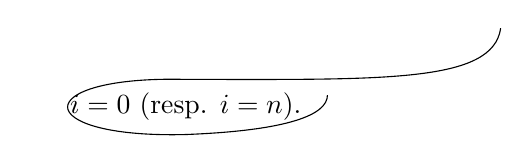
\begin{tikzpicture}
\node at (0,0) {$i=0$ (resp. $i=n$).};
\draw (4,1) .. controls (3.9,.3) and (2.5,.35) .. (0,.35) .. controls (-2,.4) and (-2,-.4) .. (0,-.35) .. controls (1.3,-.3) and (1.8,-.1) .. (1.8,.15);
\end{tikzpicture}}

b') Énoncé dual

c) $H^{\unsure{i-2}}(Q^{n-1})(-1)\longrightarrow H^i(Q^n)$ est
\[
\left|\begin{array}{l}
\left.\begin{array}{l}
\text{bijectif si }\deleted{\unsure{i\neq0,2}}\inserted{i\geq2},\ i\neq n\\
\text{injectif pour tt }i
\end{array}\right\}(n\text{ \uline{pair}})\\[2pt]
\left.\begin{array}{l}
\text{bijectif si }i\geq2,\ i\neq n+1\\
\text{surjectif pour tt }i\geq1
\end{array}\right\}(n\text{ impair})
\end{array}\right.
\]
\unsure{d'|c'}) Énoncé dual: $H^i(Q^n)\longrightarrow H^i(Q^{n-1})$ est
\[
\left|\begin{array}{l}
\left.\begin{array}{l}
\text{bijectif si }i\leq2n-2,\ i\neq n\\
\text{surjectif pour tt}
\end{array}\right\}n\text{ \uline{pair}}\\
\left.\begin{array}{l}
\text{bijectif si }i\leq2n-2,\ i\neq n-1\\
\text{injectif pour tt }i\leq2n-1
\end{array}\right\}n\text{ impair}
\end{array}\right.
\]
d) $H^{\unsure{i|2i}}(Q^n)$ \deleted{de rang} est de rang $1$ en toute dimension \inserted{paire} \uline{sauf} pour $n$ pair et \deleted{\unsure{2}} $i=n$, où il est de rang $2$.

e) Si $n$ pair,

\margin{
\diagram{\begin{tikzcd}[column sep=large,row sep=large]
\unsure{F}\\
X\arrow[dr,no head]\arrow[r,phantom,"\subset" description]&X'=Y[\unsure{h,-1_h|h,1/h}]\arrow[d,no head]\\
&Y
\end{tikzcd}}
}
\mspage{21}

\scanpage{23}
\mspage{23}
multiplicatif \deleted{\unsure{autre}} sauf le groupe unité. Comme un sous-groupe d'un groupe de type multiplicatif est de type multiplicatif (Exp VI\quad), il s'ensuit que \deleted{tout} pour tout sous-groupe de type multiplicatif $H$ de $G/Z_0$, on a $H\cap G/Z_0=0$, donc $H\longrightarrow G/G_0$ est injectif. Comme $G/G_0$ est un groupe algébrique radiciel, donc fini sur $k$, cela implique que $H$ est lui-même radiciel et de \uline{rang majoré} par celui de $G/G_0$. Cela \inserted{implique} que la famille des sous-groupes de type multiplicatifs de $G$ admet un plus grand élément, soit $Z$.

Je dis que $G/Z$ n'a pas de sous-groupe de type multiplicatif autre que le sous-groupe unité. Cela résulte du fait (démontré dans Exp VII\quad) qu'une extension commutative de deux groupes algébriques de type multiplicatif est de type multiplicatif; \deleted{compte tenu du caractè-} si donc $Z'$ est l'image inverse dans $G$ d'un sous-groupe de type multiplicatif de $G/Z$, alors $Z'$ est de type multiplicatif, donc $Z'=\unsure{Zc|Z}$ par le caractère maximal de $Z$, donc $Z'/Z=0$.

Il résulte maintenant aisément du ``principe de l'extension finie'' que pour toute extension $K$ de $k$, $(G/Z)_K=G_K/Z_K$ n'a pas non plus de sous-groupe de type multiplicatif sauf le groupe unité.

Nous pouvons maintenant prouver que $Z$ est un centre réductif de $G$. En effet, soit $u:H\longrightarrow G_S$ un homomorphisme de $S$-groupes, où $S$ est un préschéma sur $k$ et $H$ un groupe de type multiplicatif et de type fini sur $S$, prouvons que $u$ se factorise à travers $Z_S$. Il revient au même de dire que l'homomorphisme composé $H\longrightarrow G_S\longrightarrow(G/Z)_S=G_S/Z_S$ est nul. Or je dis que, posant $U=G/Z$, tout homomorphisme $u:H\longrightarrow U_S$ est nul. En effet, en vertu de Exp IX 5.2. on est ramené au cas où $S$ est le spectre d'un corps, et par Exp IX 6.8. cela résulte alors du

\mspage{22}

\scanpage{24}
\[
\unsure{P|\mathbb P}^1\times P^1\simeq Q^2\subset Q^1\simeq P^1
\qquad \frac{n-1}{2}+1=\frac{n+1}{2}
\]
\[
\unsure{\cdot|0}\unsure{\text{---}|\longrightarrow}H^0(Q^1)\longrightarrow H^2(
\]
\[
H^2(Q^n)\text{---}H^{2\nu-2}(Q^n)
\qquad\margin{n=2\nu}
\]
\[
\xi^0\text{---}\xi^{\nu-1}\quad\xi^\nu\quad\overset{\deleted{\unsure{\varphi}}}{\xi^{\nu+1}}\inserted{\tfrac12}\text{---}\xi^{2\nu}
\]
\[
\ell
\]
\[
\deleted{\unsure{\xi^1_2\text{---}\xi_\nu\quad\xi}}
\]
\[
Q^n\quad\left\{\begin{array}{l}
\xi_i\in H^{2i}(Q^n,\mu(i))\qquad\deleted{0\leq i\ \unsure{\nu}\leq2n}\\
\deleted{\lambda_{\unsure{2\nu}}\in H^{2\nu}(Q^{2\nu})}\quad
\lambda_{2\nu}\in H^{2\nu}(Q^{2\nu})
\end{array}\right.
\]
\[
\deleted{\unsure{Q}}\qquad \unsure{\xi_i}
\]
\diagram{\begin{array}{ccc}
Q^{n-1}&\subset&Q^n\\
\xi_{\unsure{i}}&\longleftarrow&\xi_i\\
\xi_i&\rightsquigarrow&\xi_{i+2}
\end{array}}
\[
\begin{pmatrix}1,&1\\1,&-1\end{pmatrix}
\]
\diagram{\begin{array}{ccccccccc}
Q^0&\subset&Q^1&\subset&Q^2&\subset&Q^3&\subset&Q^4\\
\lambda_0,\xi^0&&\xi^0&&\xi^0&&\xi^0&&\xi^0\\
&&\frac12\xi&&(\lambda_2,\xi)&&\xi&&\xi\\
&&&&\frac12\xi^2&&\frac12\xi^2&&(\lambda_4,\xi^2)\\
&&&&&&\frac12\xi^3&&\frac12\xi^3\\
&&&&&&&&\frac12\xi^4
\end{array}}
\[
\deleted{\unsure{Q^{2\nu}}}:\qquad\deleted{\unsure{\xi}}\ldots
\]
\margin{d'indice $2$ dans $H^{2\nu}(Q^{2\nu})$, \unsure{si on prend} $\frac12(\xi^\nu+\lambda_\nu)=\varphi_\nu$, \unsure{on a une base} $(\xi^\nu,\varphi_\nu)$}
\diagram{\[
\boxed{\begin{array}{ll}
Q^{n=2\nu}:&\xi^0,\ldots,\xi^{\nu-1},[\xi^\nu,\lambda_\nu],\frac12\xi^{\nu+1},\ldots,\frac12\xi^{2\nu}\\
Q^{n=2\nu+1}:&\xi^0,\ldots,\xi^\nu,\frac12\xi^{\nu+1},\ldots,\frac12\xi^{2\nu+1}
\end{array}}
\]}
\margin{$\lambda_\nu$}
\mspage{23}

\scanpage{25}
\mspage{\unsure{10|19}}
\deleted{\unsure{de $R$}. En vertu de 10.5.3. c'est un sous-groupe fermé de $G$ lisse sur $S$, donc \unsure{l'assertion affirmée}, et comme $T$ est central, on a \unsure{$R\subset H$}.}

Ceci résulte du \deleted{résultat suivant}

\uline{Lemme} 1.14. Soient $G$ \deleted{affine}\inserted{un $S$-préschéma en groupes,} de présentation finie sur $S$, $T$ un tore maximal de $G$, \deleted{alors $T$ contient tout sous-tore central} $R$ un sous-tore de $G$, et supposons que $T$ et $R$ commutent. Alors $R\subset T$.

En effet, comme $R$ et $T$ commutent, le morphisme $R\times_S T\longrightarrow G$ défini \deleted{\unsure{par}} par $(r,t)\rightsquigarrow r.t$ est un homomorphisme de groupes, donc en vertu de 1.8. il admet un sous-groupe image $T'$ dans $G$, qui est un \deleted{sous-}groupe de type multiplicatif quotient de $R\times_S T$, donc un tore, contenant évidemment $T$. Comme $T$ est un tore maximal, on a $T'=T$ (1.4.), donc $R\subset T$, \deleted{cqfd} ce qui démontre 1.14. donc 1.13. En particulier, \inserted{utilisant 6.7. b):}

\uline{Corollaire} 1.15. Soit $G$ un $S$-préschéma en groupes \deleted{\unsure{affi}} \uline{commutatif}, lisse et affine sur $S$, \inserted{de rang réductif localement constant.} Alors $G$ admet un unique tore maximal, et ce\deleted{\unsure{ci}} \deleted{\unsure{sous-tore de plus}} dernier contient tout sous-tore de $G$.

\uline{Corollaire} 1.16. Soit $G$ un $S$-préschéma en groupes, lisse et affine sur $S$. Supposons que pour tout $s\in S$, désignant par $\bar s$ le spectre d'une clôture algébrique \inserted{$k$} de $k(s)$, la fibre géométrique $G_{\bar s}$ soit un groupe algébrique connexe, et nilpotent (au sens de BIBLE, i.e. le groupe $G(k)$ de ses points à valeurs dans $k$ est nilpotent). \inserted{Supposons de plus le rang réductif de $G$ loc.constant.} Alors $G$ admet un unique tore maximal $T$, \inserted{de plus} $T$ est central et c'est le plus grand sous-tore de $G$.

En vertu de 1.7. b), $G$ admet localement pour fpqc un tore maximal, et en vertu de 1.13. on est ramené à prouver qu'un tore maximal de $G$ est central. En vertu de Exp \inserted{$\overline{\underline{\mathrm{IX}}}$}\deleted{\unsure{XI}}, 5.6. b), on est ramené au cas où $S$ est le spectre d'un corps, qu'on peut supposer algébriquement clos.
\mspage{24}

\scanpage{26}
\[
Q^i\subset Q^j\qquad\xi
\]
\[
\deleted{\mathbb Z[T][T']/T^{2\nu+2},\ 2T'-T^{\nu+1}}
\]
\diagram{\[
\left\{\begin{array}{l}
\xi^0,\ldots,\xi^{\nu-1},[\xi^\nu,\lambda_\nu],\xi_{\nu+1},\ldots,\xi_{2\nu}\\
\xi^0,\ldots,\xi^\nu,\xi_{\nu+1},\ldots,\xi_{2\nu+1}
\end{array}\right.
\]}
\margin{\[
\begin{array}{l}
\left[\begin{array}{l}
2\xi_i=\xi^i\\
\xi^i_{\deleted{\unsure{i}}}\xi_j=\xi_{i+j}\\
\xi_i\xi_j=0\quad\text{pour raisons de degré}
\end{array}\right.\\
\left[\begin{array}{l}
\lambda_\nu^2=2\xi_{2\nu}=\xi^{2\nu}\\
\lambda_\nu\xi=0
\end{array}\right.\\
\left[\begin{array}{l}
\lambda_\nu\xi_\alpha=0\quad\alpha\geq\nu+1\\
\text{raisons de degré}
\end{array}\right.
\end{array}
\]}
\diagram{\begin{array}{l}
\begin{array}{ccc}
Q^i&\subset&Q^j\qquad(i\leq j)\\
\xi^\alpha&\underset{\deleted{\unsure{\xi}}}{\longleftarrow}&\xi^\alpha\\
\xi_\alpha&\leftsquigarrow&\xi_\alpha
\end{array}\\
\left.\begin{array}{ccc}
0&\leftsquigarrow&\lambda_\nu\\
\xi_\nu&\leftsquigarrow&\varphi_\nu
\end{array}\right\}\text{si }i<j=2\nu
\end{array}}
\margin{: $\lambda_\nu$ est une \uline{classe \unsure{effaçable}}}
\diagram{\begin{array}{l}
\begin{array}{ccc}
\xi^\alpha&\rightsquigarrow&\xi^{\alpha+(j-i)}\\
\xi_\alpha&\rightsquigarrow&\xi_{\alpha+(j-i)}
\end{array}\\
\left.\begin{array}{ccc}
\lambda_\nu&\rightsquigarrow&0\\
\varphi_\nu&\rightsquigarrow&\xi_{\nu+(j-i)}
\end{array}\right\}\text{si }i=2\nu<j
\end{array}}
\margin{: $\lambda_\nu$ est une classe ``évanescente''.}
\mspage{25}

\scanpage{27}
\mspage{21}
\margin{\unsure{03}}
finie, \inserted{et à fibres affines,} $Z$ un sous-préschéma en groupes. Pour que $Z$ soit un centre réductif de $G$, il faut et il suffit qu'il soit de type multiplicatif, et que pour tout $s\in S$, \deleted{désignant par} $Z_s$ soit un centre réductif de $G_s$.

En effet, il résulte d'abord de Exp IX 5.6. b) qu'alors $Z$ est central. Comme les conditions envisagées sont stables par changement de base, il reste à prouver que tout homomorphisme central $u:H\longrightarrow G$, avec $H$ de type multiplicatif et de type fini, se factorise par $Z$. Or, $Z$ étant central, $u$ et l'immersion canonique $v:Z\longrightarrow G$ définissent un homomorphisme de groupes
\[
w:H\times_S Z\longrightarrow G.
\]
En vertu de Exp IX 6.8. ce dernier admet un groupe image $K$, qui est un sous-groupe de type multiplicatif de $G$, et tout revient à prouver que l'on a $K=Z$. Or cela est vrai fibre par fibre d'après l'hypothèse sur $Z$, et il suffit maintenant d'appliquer Exp IX 5.1. bis, \inserted{ce qui achève de prouver 4.3.}

\margin{\figure{\begin{tikzpicture}\draw (0,0)--(.7,.08)--(.7,.45)--(1.4,.45);\end{tikzpicture}}}
On notera que dans le critère 4.3., l'hypothèse que pour tout $s\in S$, $Z_s$ soit un centre réductif de $G_s$ est en fait purement géométrique, i.e. il suffit de le vérifier sur la clôture algébrique de $k(s)$, comme il résulte de la deuxième assertion 4.2.

\margin{\unsure{al}}
\margin{\figure{\begin{tikzpicture}\draw (0,0) .. controls (.2,.55) and (.35,.6) .. (.6,.35);\end{tikzpicture}}}
\uline{Théorème} 4.4. Soit $G$ un groupe algébrique \uline{affine} sur un corps $k$. Alors $G$ admet un centre réductif.

Comme le centre de $G$ est représentable par un sous-groupe fermé de $G$ (Exp VIII 6.7.), on est ramené aussitôt au cas où $G$ est commuta\deleted{\unsure{tif}}tif. De plus, en vertu de 4.2. on peut supposer $k$ algébriquement clos. Nous verrons \deleted{\unsure{ailleurs}}\inserted{dans Exp $\overline{\underline{\mathrm{XIII}}}$} que dans ce cas $G$ s'écrit comme un produit \deleted{\unsure{de}} $Z\times U$, où $Z$ est de type multiplicatif, et $U$ ``unipotent'', d'où il résultera aussitôt que $Z$ est bien un centre réductif de $G$. Nous allons
\mspage{26}

\scanpage{28}
\[
\begin{bmatrix}1,&1\\1,&-1\end{bmatrix}
\]
\diagram{\begin{array}{ccccccc}
Q^0&Q^1&Q^2&Q^3&Q^4&Q^5&Q^6\\
{[\lambda_0,\xi^0]}&\xi^0=1&\xi^0=1&\xi^0=1&\xi^0=1&\xi^0=1&\xi^0=1\\
&\frac12\xi^{\deleted{\unsure{0|1}}}&[\lambda_1,\xi]&\xi&\xi&\xi&\xi\\
&&\frac12\xi^2&\frac12\xi^2&[\lambda_2,\xi^2]&\xi^2&\xi^2\\
&&&\frac12\xi^3&\frac12\xi^3&\frac12\xi^3&[\lambda_3,\xi^3]\\
&&&&\frac12\xi^4&\frac12\xi^4&\frac12\xi^4\\
&&&&&\frac12\xi^5&\frac12\xi^5\\
&&&&&&\frac12\xi^6
\end{array}}
\margin{\deleted{a) Cohomologie de $Q^n$ nulle en dim impaire}}
\mspage{27}

\scanpage{29}
\mspage{\unsure{12}}
Alors $T(k)$ est dans le centre de $G(k)$ en vertu de BIBLE 6. th.2, ce qui implique que $T$ est dans le centre de $G$, \deleted{en vertu de Exp \unsure{VI}}\inserted{car $\underline{\operatorname{Centr}}_G(T)$ est un sous-schéma fermé de $G$ (Exp $\overline{\underline{\mathrm{VIII}}}$ 6.6.) qui contient les points de $G(k)$, donc est identique à $G$ par le Nullstellensatz, ($G$ étant réduit).}
\margin{\figure{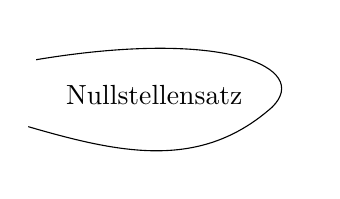
\begin{tikzpicture}
\node at (0,0) {Nullstellensatz};
\draw (-1.5,.45) .. controls (.9,.85) and (2,.35) .. (1.5,-.15) .. controls (.6,-.95) and (-.4,-.75) .. (-1.6,-.4);
\end{tikzpicture}}}

Enfin, pour référence ultérieure, signalons la proposition triviale suivante, (dont nous avons fait déjà usage implicitement):

\uline{Proposition} 1.17. Soient $G\supset H\supset T$ des préschémas en groupes de type fini sur $S$. \deleted{Alors}\inserted{Conditions équivalentes:}

(i) \deleted{Si} $T$ est un tore maximal de $G$, \deleted{c'est un tore maximal de $H$, et \unsure{pour tout $s\in S$ $T_s$ est un tore maximal de $G_s$}}

(ii) \deleted{Si} $T$ est un tore maximal de $H$, et \deleted{si} pour tout $s\in S$, on a égalité des rangs réductifs $\rho_r(G_s)=\rho_r(H_s)$, \deleted{alors $T$ est un tore maximal de $G$}.

2. \uline{Le groupe de Weyl.}

Soit d'abord $k$ un corps algébriquement clos, et soit $G$ un groupe algébrique sur $k$, \inserted{lisse et affine sur $k$.} Si $T$ est un tore maximal, $C$ son centralisateur et $N$ son normalisateur, alors en vertu de \inserted{Exp $\overline{\underline{\mathrm{XI}}}$} 5.9. ce sont des sous-groupes fermés lisses de $G$, \deleted{\unsure{essentiellement}} et $C$ est un sous-groupe ouvert de $N$, de sorte que \inserted{$W=$} $N/C$ est un groupe fini \deleted{\unsure{(et même, qui sera appelé le groupe de Weyl}}\inserted{étale sur $k$, donc déterminé par le groupe $W(k)$} de \deleted{$G$ relativement au tore maximal $T$}. ses points à valeurs dans $k$, comme $W=W(k)_k$ (groupe constant défini par le groupe fini ordinaire $W(k)$). Le groupe fini $W(k)$ s'appelera le \uline{groupe de Weyl géométrique}, (ou simplement groupe de Weyl si une confusion n'est pas à craindre), \uline{de} $G$ \uline{relativement à} $T$. En vertu du théorème de \inserted{conjugaison de} Borel, les groupes de Weyl relatifs aux divers tores maximaux sont isomorphes entre eux, c'est pourquoi on parle parfois ``du'' groupe de Weyl de $G$, sans préciser de tore maximal. \deleted{\unsure{On}} Comme la formation de $C,N$, et $N/C$ commute à toute extension de la base, on voit que si $k'$ est une extension algébriquement close de $k$, le groupe de Weyl géométrique de $G_{k'}$ relativement à $T_{k'}$ est canoniquement \unsure{isomorphe}
\mspage{28}

\scanpage{30}
\[
\deleted{\boxed{\text{\textcircled{F}}\otimes G}}
\qquad
L.(F)\otimes L.(G)=(F\underline{\underline{\otimes}}G)
\]
\margin{\figure{\begin{tikzpicture}
\node[anchor=west] at (.2,4) {$n=2\nu$};
\draw (0,4.4)--(-.1,2.4);
\draw[->] (-.12,1.9) .. controls (-.2,1.5) and (-.25,.3) .. (-.3,0);
\end{tikzpicture}}}
\diagram{\begin{tikzcd}[column sep=large,row sep=large]
H^{n+1}(U^{n+1})(1)
\arrow[r,"\mathrm{inj}","\partial"']
\arrow[rr,bend left=35,"{\deleted{\unsure{bij}}\ \mathrm{bij}\ \uline{exc.\ 2},\ \ell^{(2\nu+1)}\rightsquigarrow2\ell^{(2\nu)}}"]
&H^n(Q^n)\arrow[r,"\mathrm{surj}"]&H^n(U^n)\\
\ell^{2\nu+1}\arrow[r,rightsquigarrow]&\lambda_\nu\\
&{[\lambda_\nu,\xi^\nu]}\arrow[r,rightsquigarrow]&{[2\ell_{\deleted{\unsure{2\nu}}}^{2\nu},0]}\\
&\varphi_\nu=\frac12(\lambda_\nu+\xi^\nu)\arrow[r,rightsquigarrow]&\ell_{\deleted{\unsure{2\nu}}}^{2\nu}
\end{tikzcd}}
\margin{$0\text{---}$}
\[
\ell_{\deleted{\unsure{2\nu+1}}}^{2\nu+1}
\]
\[
\deleted{H^n(Q^n)\longleftarrow H^n(U^n)}
\]
\diagram{\begin{tikzcd}[column sep=large,row sep=large]
&\lambda_\nu&\ell_{2\nu}\arrow[l,rightsquigarrow]\\
H_c^{n+1}(U^{n+1})(+1)&H^n(Q^n)\arrow[l,"\mathrm{surj}","\partial"']&H_c^n(U^n)\arrow[l,"\mathrm{inj}"]\\
{[2\ell_{2\nu+1},0]}&{[\lambda_\nu,\xi^\nu]}\arrow[l,rightsquigarrow]\\
\ell_{2\nu+1}&\varphi_\nu\arrow[l,rightsquigarrow]\\
{}&&{}\arrow[ll,bend left=30]\\
2\ell_{2\nu+1}&&\ell_{2\nu}\arrow[ll,rightsquigarrow]
\end{tikzcd}}
\[
Q^{n+1}-Q^n=U^{n+1}
\]

\uline{N.B.}\quad \uline{On \unsure{interprète}} $\unsure{\varphi_\nu}$ \uline{directement par les sous-espaces isotropes maximaux.}

les deux familles de tels sous-espaces \unsure{correspondent|corresp.}: les classes $\alpha_\nu,\beta_\nu$. On a
\[
\alpha_\nu+\beta_\nu=\xi^\nu,\qquad
\alpha_\nu-\beta_\nu=\lambda_\nu,\qquad
\varphi_\nu=\alpha_\nu\text{---}
\]
\mspage{29}

\scanpage{31}
\mspage{26}
Démonstration.

a) et b). La démonstration de a) et de la première assertion dans b) est essentiellement identique à celle de 1.7. a) et b), et nous nous dispensons de reproduire ici le raisonnement. Signalons seulement qu'il faut faire appel dans a) à Exp IX 5.6. (utilisant le fait que $G$ est à fibres connexes). Prouvons la deuxième assertion de b), i.e. que si $Z$ est un centre réductif de $G$, alors $G'=G/Z$ admet pour centre réductif le sous-groupe unité. Notons tout de suite qu'en vertu de Exp VIII 5.1. le groupe quotient $G/Z$ estb bien représentable, il est affine sur $S$, de présentation finie sur $S$ (Exp VIII 5.8.) et même lisse sur $S$ (car il suffit de le voir pour les fibres, $G'$ étant plat de présentation finie sur $S$, or pour les fibres \deleted{cela est} on a signalé dans Exp VI qu'un quotient d'un groupe algébrique lisse sur un corps $k$ est lisse); enfin $G$ étant à fibres connexes, il en est de même de $G'$. Ainsi $G'$ satisfait aux mêmes hypothèses de départ que $G$. Pour voir que le sous-groupe unité de $G'$ est un centre réductif, on peut se borner si on veut au cas où $S$ est le spectre d'un corps (4.3.). Soit $Z'$ un sous-groupe central de type multiplicatif de $G'$, tout revient à prouver que $Z'$ est réduit au groupe unité. Soit $Z_1$ \deleted{soit} l'image inverse de $Z'$ dans $G$, et considérons les opérations de $Z_1$ sur $G$ induites par automorphismes intérieurs de $G$. Comme $Z$ est central, $Z$ opère \deleted{\unsure{trivi|très}} trivialement, de sorte que $Z_1$ opère par l'intermédiaire d'opérations de $Z'$ sur $G$. D'ailleurs $Z$ étant dans le centre de $G$, $Z_1^{\deleted{\unsure{'}}}$ donc $Z'$ opère trivialement sur $Z$, de plus $Z'$ étant dans le centre de $G'$, les opérations de $Z'$ dans le quotient $G/Z=G'$ \unsure{(}sont également triviales. Comme $Z$ est central, il s'ensuit aussitôt que les opérations de $Z'$ sur $G$ proviennent d'un
\mspage{30}

\scanpage{32}
\[
Q^{2\nu}:\quad \xi:\ H^{2i}(\deleted{\unsure{\xi_2|\xi_\nu}}Q^{2\nu})
\text{---}H^{2i+2}(\deleted{\unsure{\xi_2|\xi_\nu}}Q^{2\nu})(1)
\]
\deleted{\uline{injectif} si $\unsure{2i<2\nu}$ i.e. $i\leq\nu-1$}
    
\uline{bijectif} si $i\neq\nu-1,\nu$
\margin{\deleted{$\unsure{i\geq0}$} ($0\leq i\leq2\nu-1$)}

$i=\nu-1$ : \uline{injectif} \deleted{si $i=\unsure{\nu+1}$}, conoyau libre de base $\unsure{\varphi_\nu|\alpha_\nu}$

$i=\nu$\qquad \deleted{\unsure{surjectif}}\inserted{\uline{surjectif}}, noyau libre de base $\lambda_\nu$

\figure{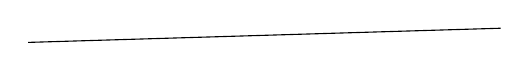
\begin{tikzpicture}\draw (0,0)--(6,.18);\end{tikzpicture}}
\[
Q^{2\nu+1}\qquad \xi:\ H^{\unsure{2i|i}}(Q^{2\nu+1})\text{---}
H^{2i+2}(Q^{2\nu\inserted{\text{\textcircled{$+1$}}}})(1)
\]
\margin{($0\leq i\leq2\nu$)}

\uline{bijectif} si $i\neq\nu$

injectif de conoyau $\mathbb Z/2\mathbb Z$ si $i=\nu$
\figure{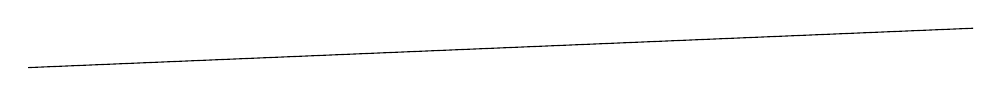
\begin{tikzpicture}\draw (0,0)--(12,.5);\end{tikzpicture}}
\mspage{31}

\scanpage{33}
\mspage{\unsure{37|31}}
En effet, on peut supposer $k$ algébriquement clos, de sorte que $T$ est contenu dans un tore maximal\deleted{\unsure{max}} $T'$. Soit $C'$ le centralisateur de ce dernier, alors on a $C'\subset C$, donc $\dim C'\leq\dim C$, cqfd.

b) \deleted{Le raisonnement de a) nous montre que} Si $\rho_r$ est localement constant, alors pour tout tore $T$ dans $G$, \deleted{et} et tout $s\in S$, si $T_s$ est \inserted{tore} maximal dans $G_s$, alors il existe un voisinage ouvert $U$ de $s$ tel que $T|U$ soit tore maximal dans $G\ U$. Utilisant maintenant le raisonnement de a), on voit que \deleted{\unsure{si}} (i)$\Longrightarrow$(ii bis). D'autre part (ii bis)$\Longrightarrow$(i), car \deleted{on peut supposer $S$} lorsque $G$ admet un tore maximal $T$, alors il est évident que $\rho_r(s)=\dim T_s$ est une fonction localement constante de \deleted{\unsure{s}} $s$, or nous avons signalé au début de la démonstration de a) que la question de la continuité de $\rho_r$ était locale pour la topologie fidèlement plate. Donc (i)$\Longleftrightarrow$(ii bis), et évidemment (ii)$\Longrightarrow$(ii bis), reste à prouver l'implication inverse \inserted{(i)$\Longrightarrow$(ii)}. Pour ceci, introduisons le foncteur $F$ de \inserted{Exp $\overline{\underline{\mathrm{XI}}}$} 4.1., qui est donc un préschéma \deleted{noethérien} lisse \inserted{et séparé} sur $S$, et considérons le sous-foncteur $\unsure{\mathcal T|\tau}$ de $F$, dont la valeur \deleted{sur} pour un $S'$ sur $S$ est l'ensemble des tores maximaux dans $G_{S'}$. Utilisant la remarque précédente \deleted{que}\inserted{que, moyennant (i),} un tore dans $G_{S'}$ qui est maximal dans la fibre d'un point $s\in S'$ est maximal au dessus d'un voisinage ouvert de $s$, on voit que $\unsure{\mathcal T|\tau}$ est représentable par un sous-préschéma ouvert de $F$, et par suite est lisse \inserted{et séparé} sur $S$. Comme le morphisme structural $\unsure{\mathcal T|\tau}\longrightarrow S$ est évidemment surjectif, il admet donc \deleted{localement} une section localement au sens de la topologie étale en vertu de \inserted{Exp $\overline{\underline{\mathrm{XI}}}$} 1.10., ce qui prouve (i)$\Rightarrow$(ii).
\margin{$\unsure{\mathcal T|\tau}$}

c) C'est une conséquence immédiate de \inserted{Exp $\overline{\underline{\mathrm{XI}}}$} 5.4. bis, compte tenu du théorème de conjugaison de Borel rappelé au début du numéro.

d) Moyennant la remarque du début de la démonstration dans a), et compte tenu de b), on peut supposer qu'il existe un tore maximal $T$
\mspage{32}

\scanpage{35}
\uline{Quadriques}\quad Une base pour l'équivalence linéaire dans
$Q^{2n}$ est \unsure{formé|formée} de
\[
1,H,H^2\ldots H^{n-1},
\underbrace{S',S''}_{\text{codim }n},
HS'=HS'',\ldots H^nS'=H^nS''.
\]
\margin{On a $H^n=S'+S''$}
[$H$ est une section hyperplane dans l'immersion projective évidente;
$S'$ et $S''$ sont définis par des sous-espaces
\deleted{affines}\inserted{linéaires de \unsure{dim $n$}}
dans $Q^{2n}$, appartenant aux deux familles algébriques distinctes
de tels sous-espaces.]

Une base de $Q^{2n+1}$ est formée de
\[
1,H,\ldots H^n,\frac{H^{n+1}}2,\ldots,\frac{H^{2n+1}}2.
\]
[\unsure{où|ici} $H$ est une section hyperplane, et \unsure{où|ici} les derniers
$\frac{H^{n+1}}2\ldots\frac{H^{2n+1}}2$ correspondent aux sous-variétés
linéaires contenues dans $Q^{2n+1}$]
\figure{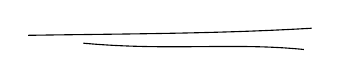
\begin{tikzpicture}
\draw (0,0) .. controls (1.3,.02) and (2.4,.02) .. (3.6,.09);
\draw (.7,-.10) .. controls (1.8,-.20) and (2.6,-.09) .. (3.5,-.18);
\end{tikzpicture}}
\mspage{34}

\scanpage{36}
\figure{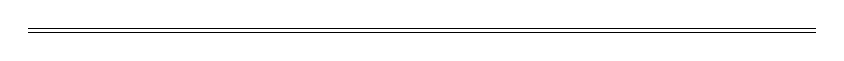
\begin{tikzpicture}\draw (0,0)--(10,0);\draw (0,-.05)--(10,-.05);\end{tikzpicture}}

\textsc{Algèbre.} --- \textit{Définition des classes de Stiefel-Whitney d'un module
quadratique sur un corps de caractéristique différente de 2.}
Note de M. \textbf{\textsc{Antoine Delzant}}, transmise par M. Jean Leray.

Soit $\mathrm A$ un corps de caractéristique différente de 2. On ne considère que
des modules quadratiques $(\mathrm E,\mathrm Q)$ $^{(1)}$, de rang fini sur $\mathrm A$,
et non dégénérés.

On désigne par $\mathrm Q^+$ l'ensemble des classes à isomorphisme près de modules
quadratiques. L'ensemble $\mathrm Q^+$ est muni de deux opérations : l'une, la somme
directe externe, définit sur $\mathrm Q^+$ une structure de monoïde abélien pour laquelle
tous les éléments sont réguliers (théorème de Witt); l'autre, le produit tensoriel,
est commutative, distributive par rapport à la précédente, et admet un élément unité
[la classe du module $(\mathrm A,\mathrm I)$, où $\mathrm I(x)=x^2$].
L'ensemble $\mathrm Q^+$ se plonge donc injectivement dans un anneau $\mathrm Q(\mathrm A)$,
qu'il engendre. L'anneau $\mathrm Q(\mathrm A)$, commutatif avec élément unité, est appelé
l'\textit{anneau des classes de formes quadratiques}. A toute classe $q$ de module
quadratique $(\mathrm E,\mathrm Q)$ on fait correspondre $\varepsilon(q)=rg(\mathrm E)$;
on définit ainsi un homomorphisme d'anneau de $\mathrm Q(\mathrm A)$ dans $\mathbf Z$
appelé l'augmentation.

Soit $\mathrm A_s$ la clôture séparable de $\mathrm A$ et $\mathrm G$ le groupe de Galois
de $\mathrm A_s$ sur $\mathrm A$; on note $\mathrm H^q(\mathrm A,\mathbf Z/2\mathbf Z)$
le $q^{\text{-ième}}$ groupe de cohomologie de $\mathrm G$ à valeurs dans
$\mathbf Z/2\mathbf Z$. On note additivement le groupe $\mathrm A^\star$,
groupe multiplicatif de $\mathrm A$, et l'on pose
$\mathrm D(\mathrm A)=\mathrm A^\star/2\mathrm A^\star$.
Le groupe $\mathrm D(\mathrm A)$ s'identifie à
$\mathrm H^1(\mathrm A,\mathbf Z/2\mathbf Z)$.

Soit $a$ un élément de $\mathrm A^\star$; on note $e_a$ sa classe dans
$\mathrm D(\mathrm A)$, et $\varphi_a$ la classe du module quadratique
$[\mathrm A,\mathrm Q;\ \mathrm Q(x)=ax^2]$.
L'élément $\varphi_a$ ne dépend que de $a$ modulo $2\mathrm A^\star$;
on peut donc définir un homomorphisme de $\mathrm D(\mathrm A)$ dans le groupe
multiplicatif $\mathrm Q(\mathrm A)^\star$ des éléments inversibles de $\mathrm Q(\mathrm A)$.
D'où un homomorphisme d'anneaux :
\[
\varphi:\quad\mathbf Z(\mathrm D)\to\mathrm Q(\mathrm A),
\]
où $\mathbf Z(\mathrm D)$ est l'algèbre de $\mathrm D(\mathrm A)$ sur $\mathbf Z$,
munie de la filtration définie par les puissances de l'idéal d'augmentation.

\textsc{Proposition.} --- \textit{L'application $\varphi$ est surjective; elle est
compatible avec les augmentations; le noyau de $\varphi$ est l'idéal engendré
par les éléments $e_a+e_b-e_{a'}-e_{b'}$, tels que
$\varphi_a+\varphi_b=\varphi_{a'}+\varphi_{b'}$.}

Le cup-produit définit une application de $\mathrm D(\mathrm A)\times\mathrm D(\mathrm A)$
dans $\mathrm H^2(\mathrm A,\mathbf Z/2\mathbf Z)$ notée $(e_a,e_b)\to a.b$.
Si l'on identifie $\mathrm H^2(\mathrm A,\mathbf Z/2\mathbf Z)$ au sous-groupe
du groupe de Brauer de $\mathrm A$ formé des $x$ tels que $2x=0$, l'élément $a.b$
\mspage{35}

\scanpage{37}
\mspage{(2)}
s'interprète comme la classe de l'algèbre de quaternions définie par le
couple $(a,b)$. Appliquant un théorème dû à Witt $^{(4)}$, on a :

\textsc{Corollaire.} --- \textit{Le noyau de $\varphi$ est l'idéal engendré par les
éléments $e_a+e_b-e_{a'}-e_{b'}$ tels que $e_{a+b}=e_{a'+b'}$ et $a.b=a'.b'$.}

Soit $\mathrm H$ un anneau gradué à degrés positifs, et
$\widetilde{\mathrm H}=\mathbf Z\times(1+\widehat{\mathrm H}^{+})$
l'anneau filtré déduit de $\mathrm H$ par le procédé exposé par Grothendieck
dans $^{(2)}$. Alors la donnée d'un homomorphisme
\[
w^1:\quad\mathrm D(\mathrm A)\to\mathrm H^1
\]
tel que $w^1(e_a)w^1(e_b)=w^1(e_{a'})w^1(e_{b'})$ dès que
$(a,b,a',b')$, vérifient les conditions du corollaire, définit un homomorphisme
d'anneau filtré de $\mathrm Q(\mathrm A)$ dans $\widetilde{\mathrm H}$.

Prenons pour $\mathrm H$ l'algèbre de cohomologie $\mathrm H(\mathrm A)$ du groupe de Galois
de $\mathrm A$ à valeurs dans $\mathbf Z/2\mathbf Z$, la multiplication étant définie par le
cup-produit. Comme $\mathrm H^1(\mathrm A,\mathbf Z/2\mathbf Z)$ s'identifie à
$\mathrm D(\mathrm A)$ on a une application
\[
w:\quad\mathrm Q(\mathrm A)\to\widetilde{\mathrm H(\mathrm A)}.
\]
L'homomorphisme $w$ définit donc des applications
\[
w^i:\quad\mathrm Q(\mathrm A)\to\mathrm H^i(\mathrm A,\mathbf Z/2\mathbf Z).
\]
Soient $(\mathrm E,\mathrm Q)$ un module quadratique et $q$ sa classe dans
$\mathrm Q(\mathrm A)$; les $w^i(q)$ sont appelées les \textit{classes de
Stiefel-Whitney} de $(\mathrm E,\mathrm Q)$ (ou de $q$).
Comme $w$ est un homomorphisme d'anneaux, on a
\[
w^n(q+q')=\sum_{i+j=n}w^i(q)w^j(q').
\]
En particulier si $q$ est la classe du module
$\left[\mathrm A^p,\mathrm Q;\ \mathrm Q(x)=\sum_1^p a_jx_j^2\right]$, on a
\[
w^1(q)=\sum a_j;\qquad w^2(q)=\sum_{i<j}a_i.a_j.
\]
On interprète $w^1(q)$ comme le discriminant de $(\mathrm E,\mathrm Q)$,
et $w^2(q)$ de la façon suivante : si $rg(\mathrm E)=p$ est pair,
soit $\mathrm C(q)$ (resp. $\mathrm C_p$) l'algèbre de Clifford de
$(\mathrm E,\mathrm Q)$ [resp. de $p(\mathrm A,\mathrm I)$].
Il existe une extension galoisienne $\mathrm B$ de $\mathrm A$ telle que
$(\mathrm E,\mathrm Q)$ et $p(\mathrm A,\mathrm I)$ soient isomorphes sur $\mathrm B$.
Donc $\mathrm C(q)$ et $\mathrm C_p$ sont isomorphes sur $\mathrm B$.
On en déduit un élément $u(q)$ du groupe de Brauer de $\mathrm A$ par le procédé
habituel $^{(3)}$, et l'on a $u(q)=w^2(q)$. Si $p$ est impair, on a la même
interprétation en remplaçant $\mathrm C(q)$ par $\mathrm C^+(q)$
(resp. $\mathrm C_p$ par $\mathrm C_p^+$) $^{(1)}$.

Enfin on vérifie que $w$ est un homomorphisme du foncteur $\mathrm Q(\mathrm A)$
dans le foncteur $\mathrm H(\mathrm A)$. Ceci provient du fait que
$\mathrm H^1(\mathrm A,\mathbf Z/2\mathbf Z)$ est un foncteur covariant en $\mathrm A$.
\mspage{36}

\scanpage{38}
\mspage{(3)}
\textit{Application aux corps de nombres algébriques.} --- Soit $\mathrm A$ un corps de
nombres algébriques; à toute valeur absolue $v$ de $\mathrm A$, on associe le
complété $\mathrm A_v$ de $\mathrm A$ pour cette valeur absolue. D'où une application
\[
\mathrm Q(\mathrm A)\to\prod\mathrm Q(\mathrm A_v)
\]
et cette application est injective (théorème de Hasse).

Si $v$ est une valuation discrète, toute classe de forme sur $\mathrm A_v$
est déterminée par $\varepsilon$, $w^1$ et $w^2$ $^{(4)}$.
Si $\mathrm A_v=\mathbf R$, le corps des réels, alors $\mathrm H(\mathbf R)$
s'identifie à $\mathbf Z/2\mathbf Z[t]$. Toute classe de forme est définie par
deux nombres entiers $m$ et $n$ ($m$, nombre de carrés positifs; $n$, nombre de
carrés négatifs).

Posant $n=\sum n_j2^j$ ($n_j=0$ ou $1$), on trouve
\[
w^j(q)=\binom nj\bmod 2;\qquad\text{en particulier}\quad w^{2^j}=n_j.
\]
Donc une classe de forme sur $\mathbf R$ est complètement déterminée par $w$.
De tout ce qui précède on déduit le diagramme commutatif suivant :
\diagram{\begin{tikzcd}
\mathrm Q(\mathrm A)\arrow[r]\arrow[d,"w"]&
\prod\mathrm Q(\mathrm A_v)\arrow[d,"(w_v)"]\\
\mathrm H(\mathrm A)\arrow[r]&\prod\mathrm H(\mathrm A_v)
\end{tikzcd}}
On démontre ainsi que l'application $w$ est injective : Sur un corps de
nombres toute classe de forme quadratique est déterminée par son rang et ses
classes de Stiefel-Whitney.

\textit{Remarque.} --- On ne sait pas si l'application
\[
\mathrm{grad}^2(\mathrm Q(\mathrm A))\to\mathrm H^2(\mathrm A,\mathbf Z/2\mathbf Z)
\]
est toujours injective, et l'on ne sait pas non plus si tout élément d'ordre 2
du groupe de Brauer de $\mathrm A$ est somme d'éléments de la forme $a.b$.

$^{(1)}$ N. \textsc{Bourbaki}, \textit{Algèbre}, chap. IX, Hermann, Paris, 1959.

$^{(2)}$ A. \textsc{Grothendieck}, \textit{Bull. Soc. math. Fr.}, \textbf{86}, 1958.

$^{(3)}$ T. A. \textsc{Springer}, \textit{Akad. Amst. Proc.}, \textbf{62 A}, 1959.

$^{(4)}$ E. \textsc{Witt}, \textit{Journal de Crelle}, \textbf{176}, 1937.
\mspage{37}

\scanpage{39}
Extrait des \textit{Comptes rendus des séances de l'Académie des Sciences},
t. 255, p. 1366-1368, séance du 10 septembre 1962.

GAUTHIER-VILLARS \& C\textsuperscript{ie},

55, Quai des Grands-Augustins, Paris (6\textsuperscript{e}),

Éditeur-Imprimeur-Libraire.

162396

Imprimé en France.
\mspage{38}

